
\section{Scalability Campaign}\label{results:scale}

Given the base parameter values described in Tables \ref{tbl:front_ref_params}
and \ref{tbl:back_ref_params}, exchanges were generated by scaling the number of
reactors in the system. The smallest system modeled included five reactors. The
largest exchanges included five-hundred reactors, a value chosen because there
are approximately five-hundred reactors currently operating (437) or under
construction (71) in the world \cite{nrxtrs}. Therefore, the largest exchanges
modeled represent a time step in a simulation in which the world-wide fleet of
reactors are all supplying or consuming a batch of fuel.

Front and back-end exchanges are explored similarly in the scalability
campaign. First, for all 18 combinations of fundamental parameters and each
solver, a set of reference cases are established, where the only varying
parameter is the number of reactors. Next, specific instance parameters are
chosen to vary in order to determine first-order effects as the exchange system
size scales. Finally, the effect of convergence criteria for the CBC solver is
investigated.

Individual figures for each experiment are provided for each fuel cycle modeled
($f_\text{fc}$) and each solver. Each figure summarizes the results for all
combinations of $f_\text{rx}$ and $f_\text{loc}$. The layout for each six-pane
figure is shown below.

\begin{figure}[h!]
  \begin{center}
    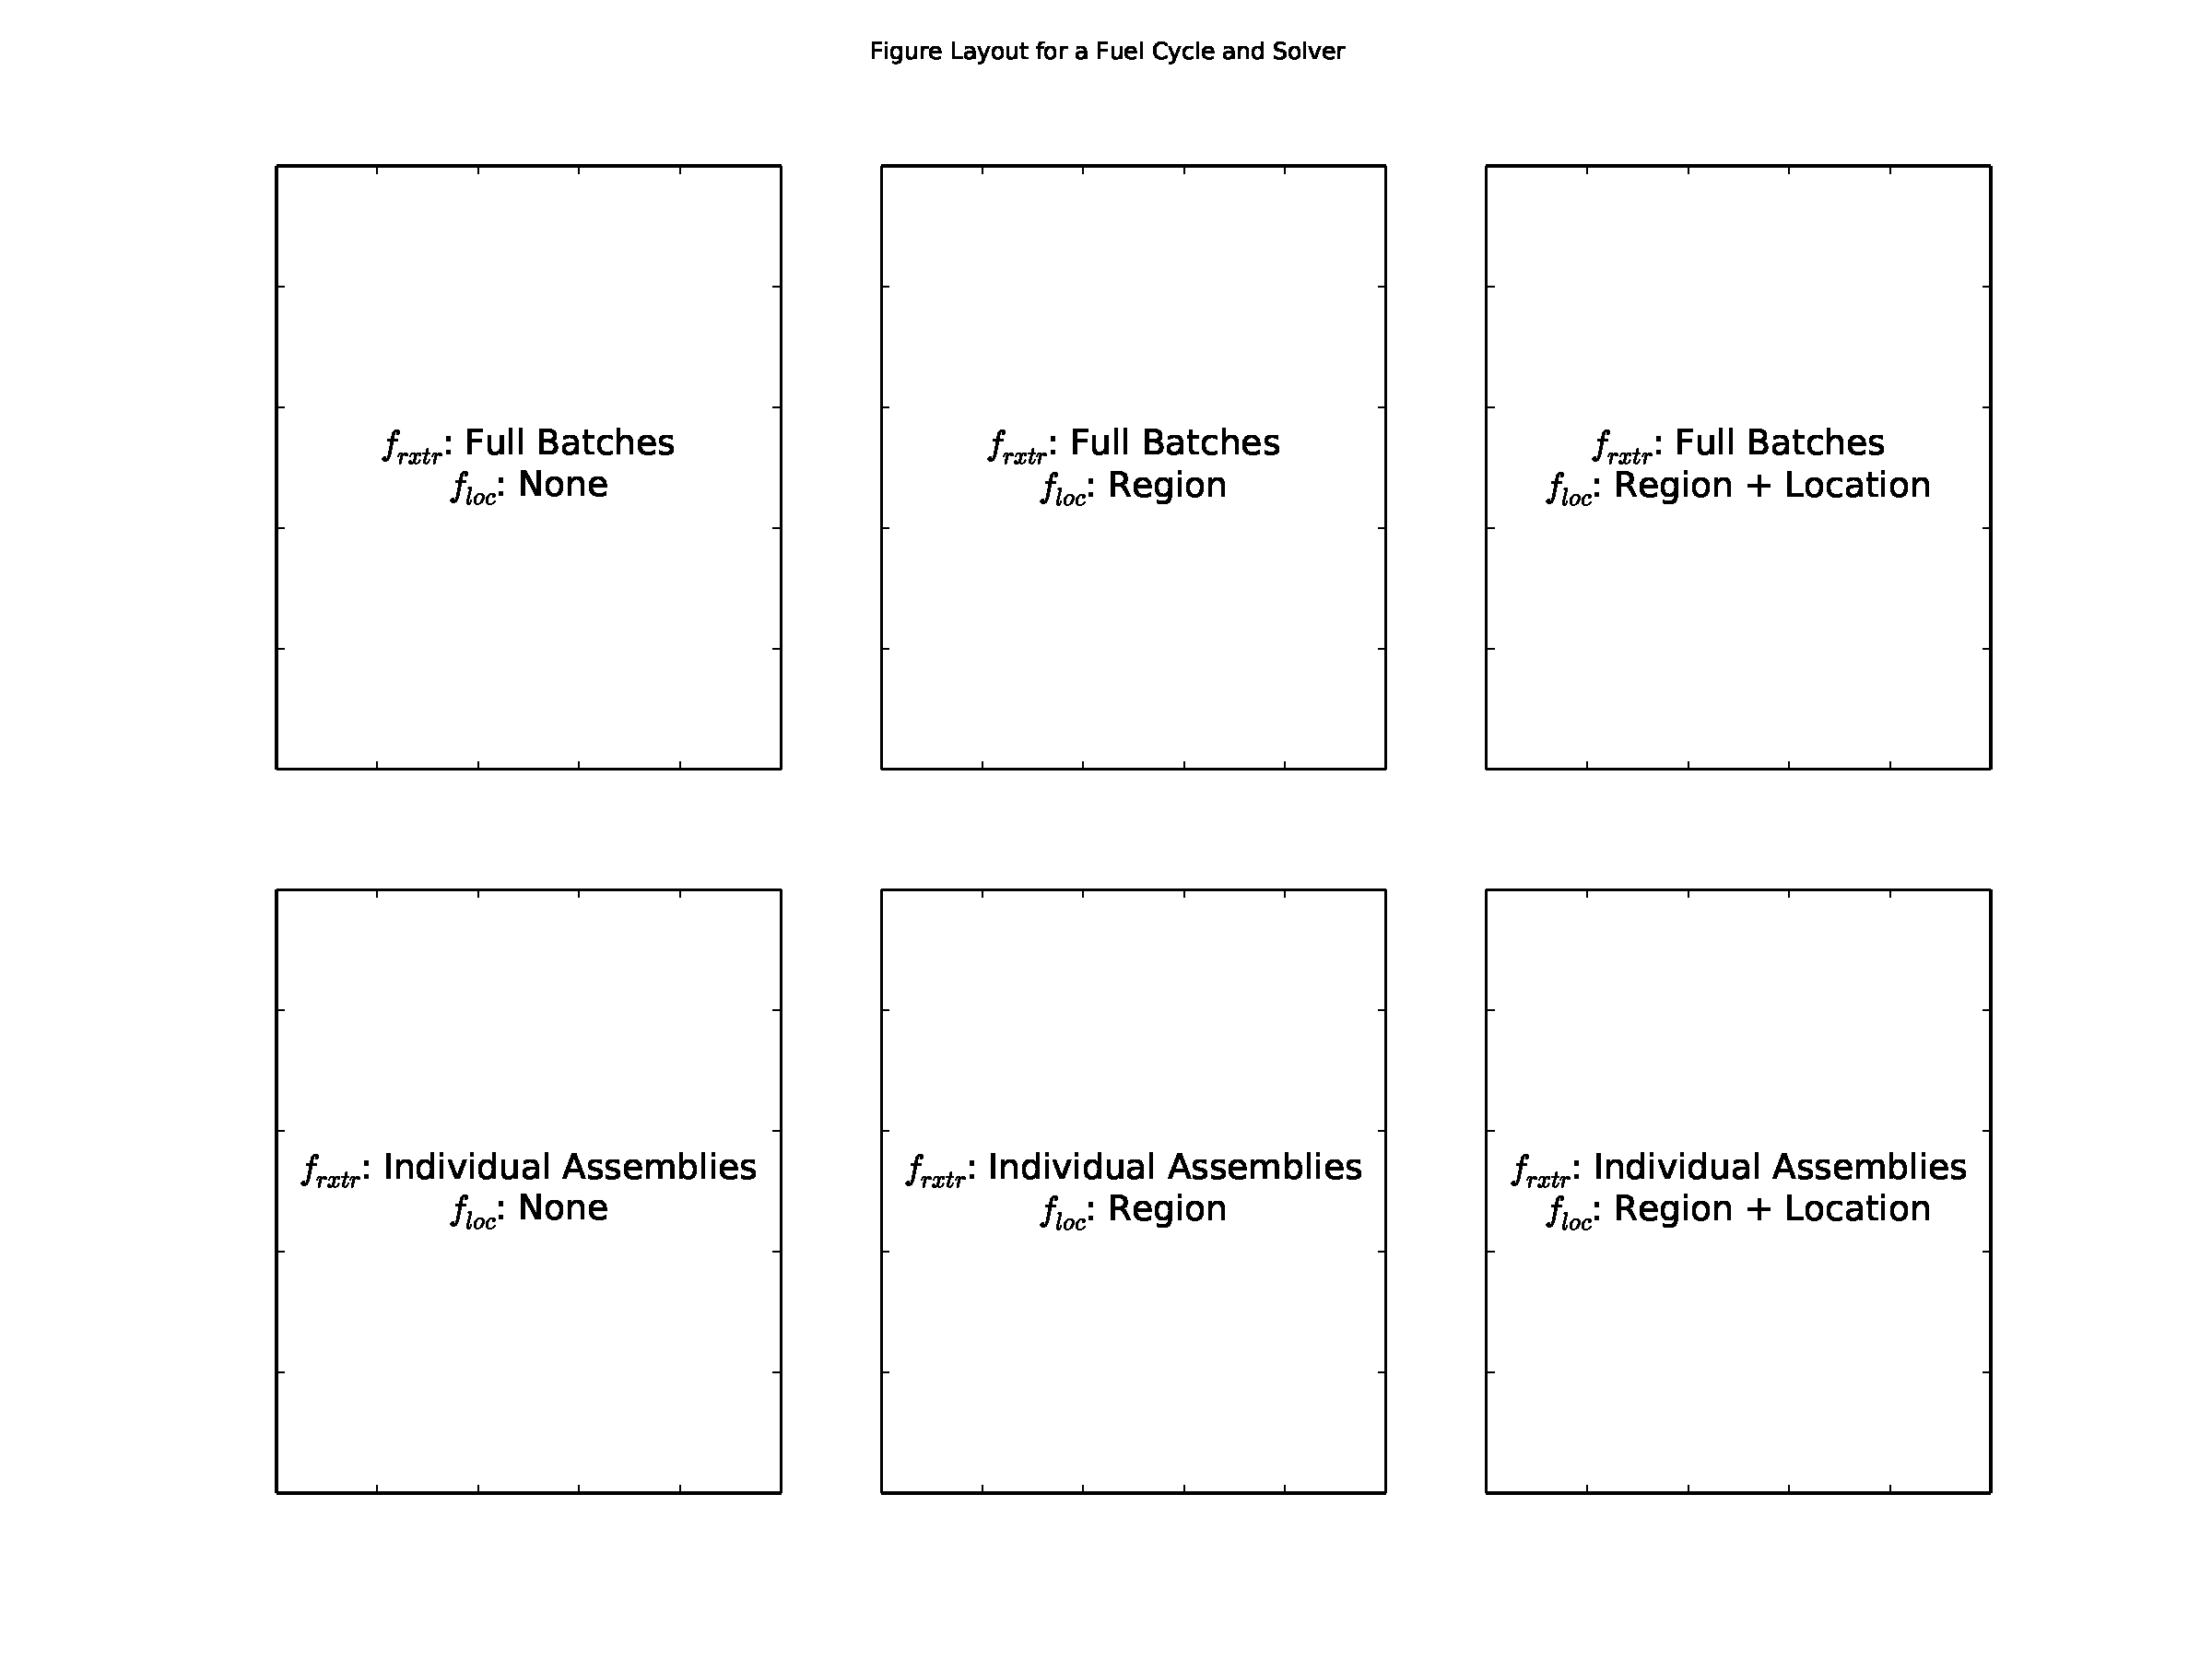
\includegraphics[width=.7\textwidth]{figure_layout.pdf}
    \caption[]{
      \label{fig:figure_layout}
      The general figure layout displaying results for different fundamental
      parameter values.}
  \end{center}
\end{figure}

\subsection{Front-End Exchanges}

\subsubsection{Reference Case}

Reference cases were generated for front-end exchanges by scaling the number of
reactors in each exchange. A step size of 5 reactors was used for the range of
$[5, 100]$ and a step size of 25 was used from $(100, 500]$. In mathematical
  programming, the number of variables and number of constraints in a problem
  are measures of problem scaling. In the NFCTP, constraints are provided by
  trading entities, and the number of variables is equal to the number of arcs
  in a given exchange graph. Accordingly, understanding how each quantiy scales
  with the number of reactors is of chief import.

Figure \ref{fig:base_front_n_rxtr_n_arcs_fc1_solvergreedy} shows how the number
of arcs scale with problem size for the MOX fuel cycle, and Figure
\ref{fig:base_front_n_rxtr_n_constrs_fc1_solvergreedy} shows the same results
for the number of constraints. The number of constraints scales linearly, for it
is a purely function of the number of entities in an exchange. However, the
number of arcs scales by $\mathcal{O}(n^2)$. During exchange generation, the
number of suppliers is a function of the number of reactors. Further, each
reactor and each supplier have an arc connecting them if the reactor can consume
the supplier's commodity. Therefore, adding a single reactor to the system
results in additional arcs for every reactor previously existing in the system,
resulting in an $\mathcal{O}(n^2)$ relationship. Both relationships hold true
regardless of the fuel cycle being modeled, and, as can be seen, are also
independent of other fundamental parameters. The arc population magnitude,
however, is a function of $f_\text{rxtr}$. As $f_\text{rxtr}$ increases, $n_a$
individual assemblies are requested rather than a single batch.

\begin{figure}[h!]
  \begin{center}
    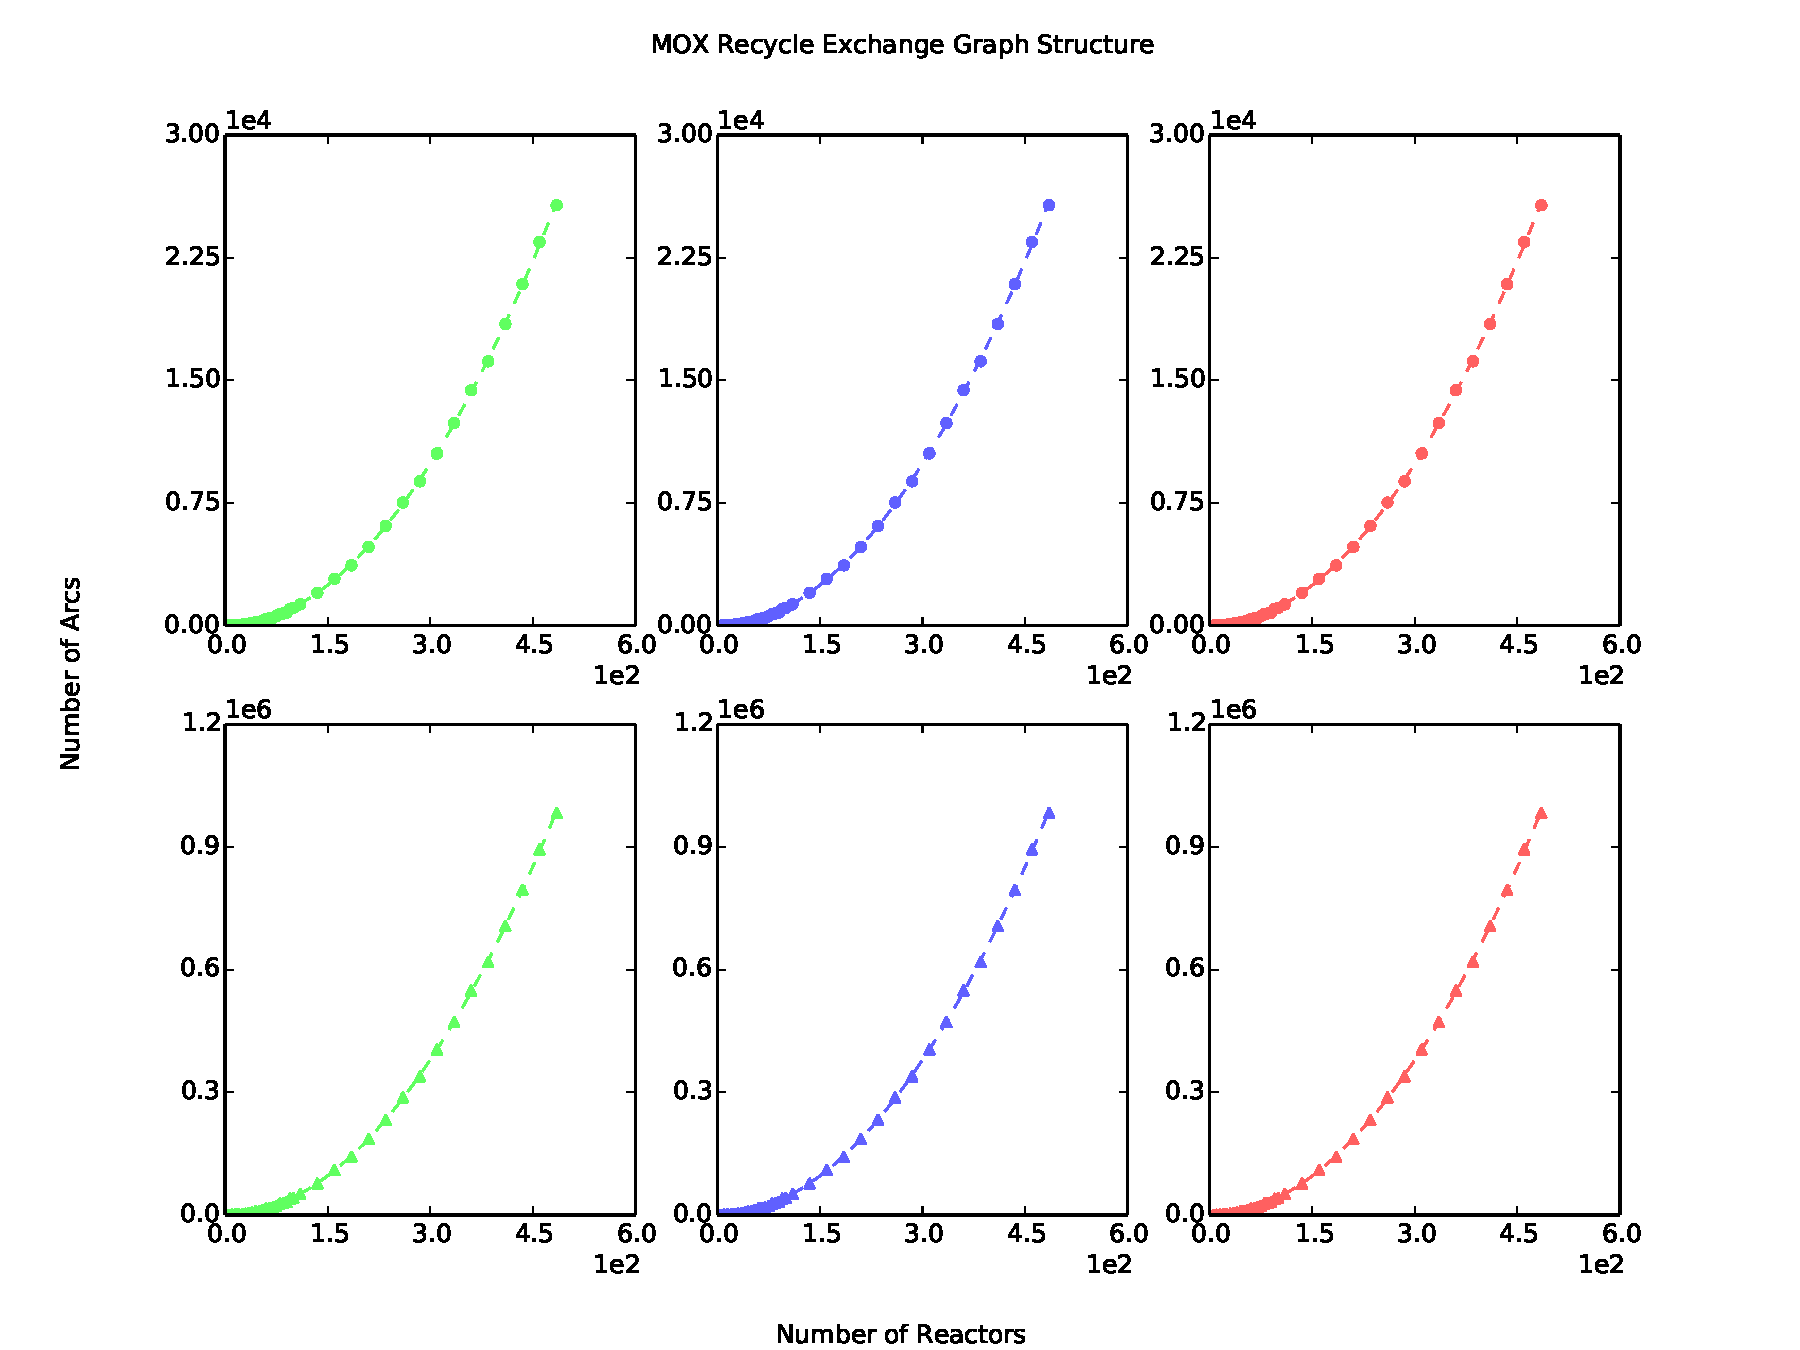
\includegraphics[width=.7\textwidth]{base_front_n_rxtr_n_arcs_fc1_solvergreedy.pdf}
    \caption[]{
      \label{fig:base_front_n_rxtr_n_arcs_fc1_solvergreedy}
      Arc population scaling with the number of reactors with coresponding linear fits.}
  \end{center}
\end{figure}

\begin{figure}[h!]
  \begin{center}
    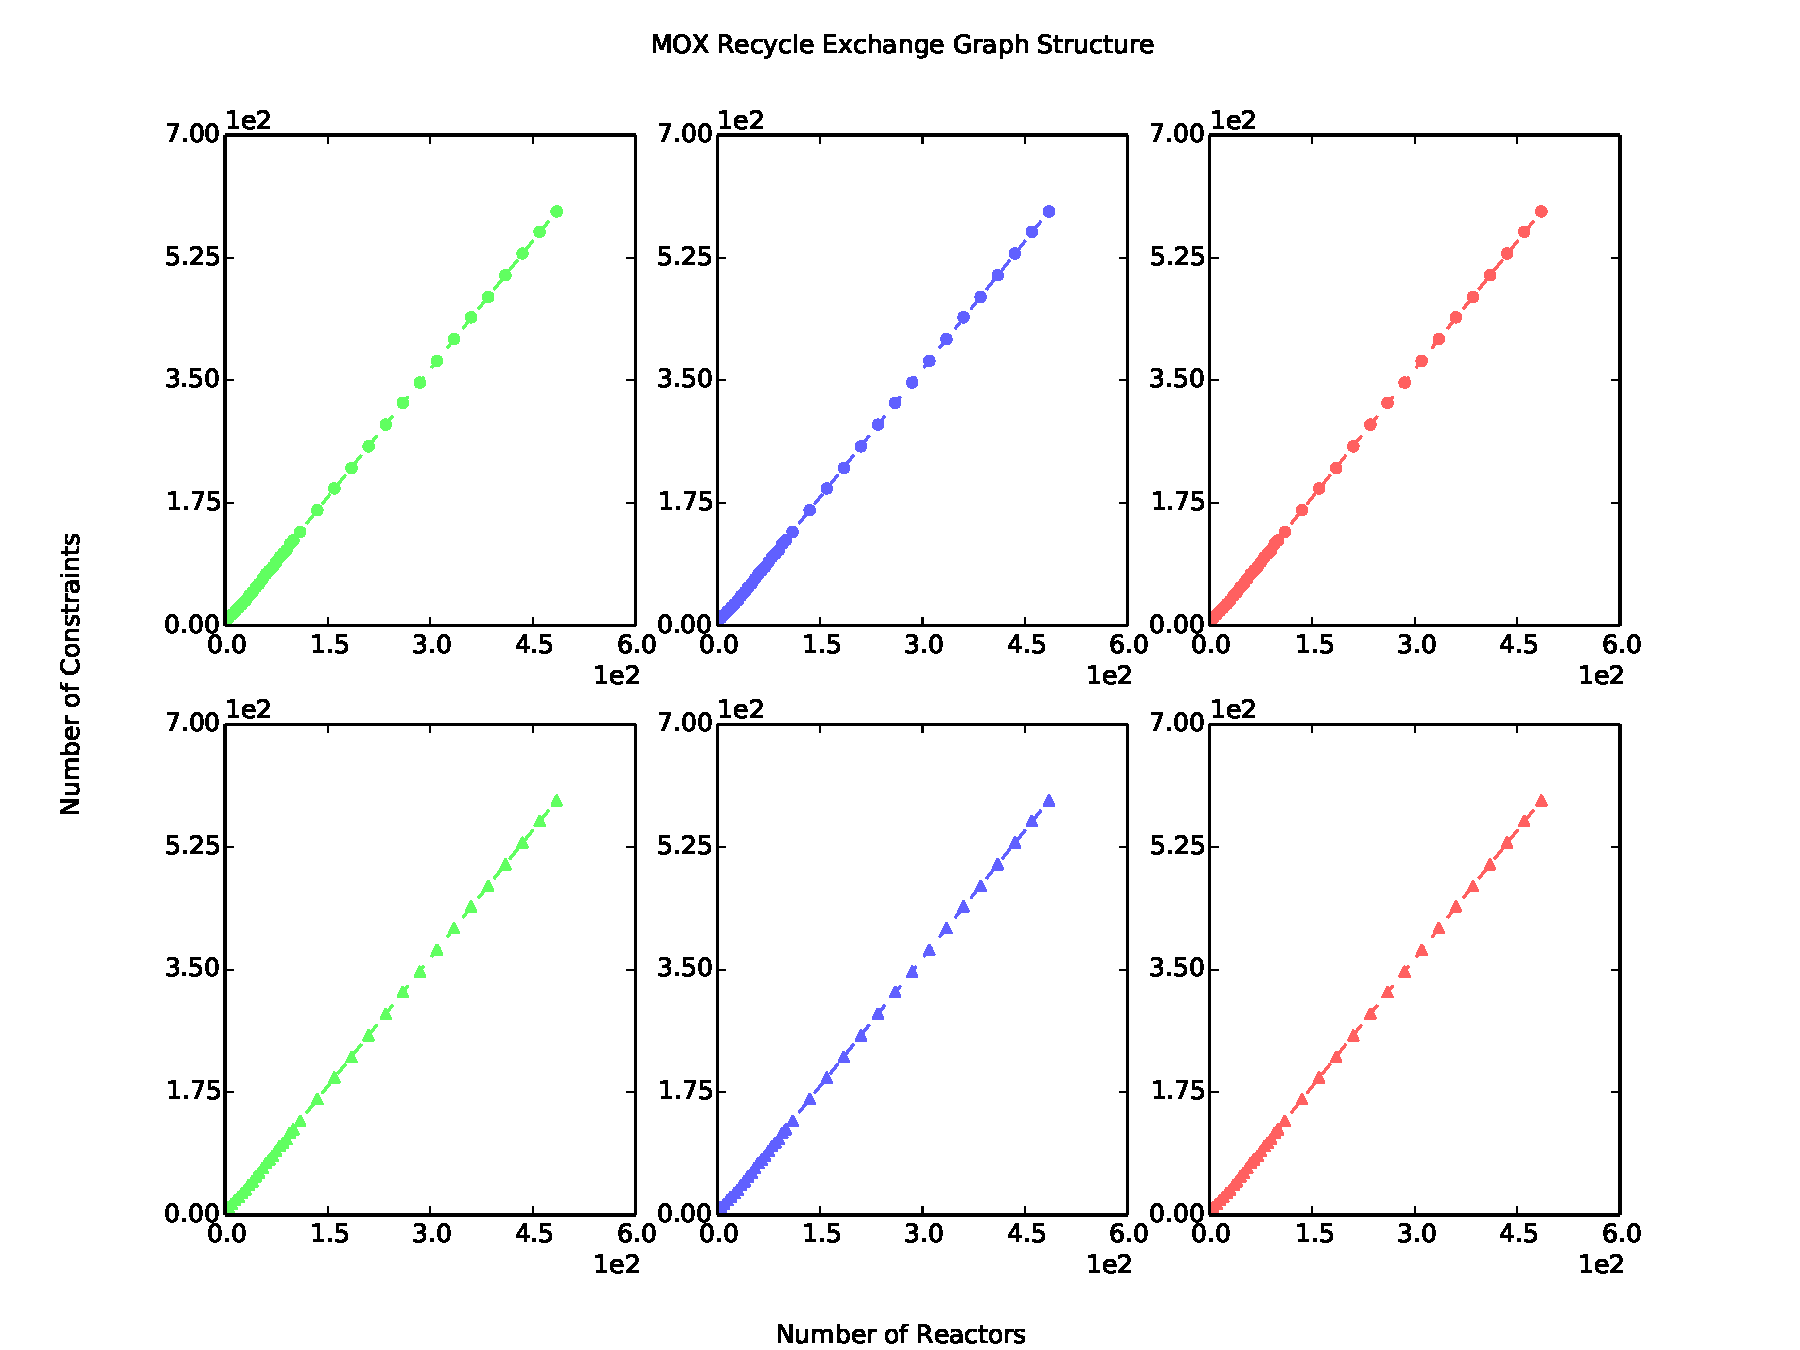
\includegraphics[width=.7\textwidth]{base_front_n_rxtr_n_constrs_fc1_solvergreedy.pdf}
    \caption[]{
      \label{fig:base_front_n_rxtr_n_constrs_fc1_solvergreedy}
      Constraint population scaling with the number of reactors with
      corresponding quadratic fits.}
  \end{center}
\end{figure}


\paragraph{Greedy Solver}

\cref{fig:base_front_n_rxtr_time_fc0_solvergreedy,fig:base_front_n_rxtr_time_fc1_solvergreedy,fig:base_front_n_rxtr_time_fc2_solvergreedy}
show the Greedy Solver results as the number of reactors increases for the OT,
MOX, and ThOX fuel cycles, respectively. Plotted with each data series is a
second-order polynomial fit, suggesting that the Greedy Solver scales as
$\mathcal{O}(n^2)$ in the number of reactors. As can be seen, this scaling is
independent of any fundamental parameter, as it is seen in every combination
thereof.

\begin{figure}[h!]
  \begin{center}
    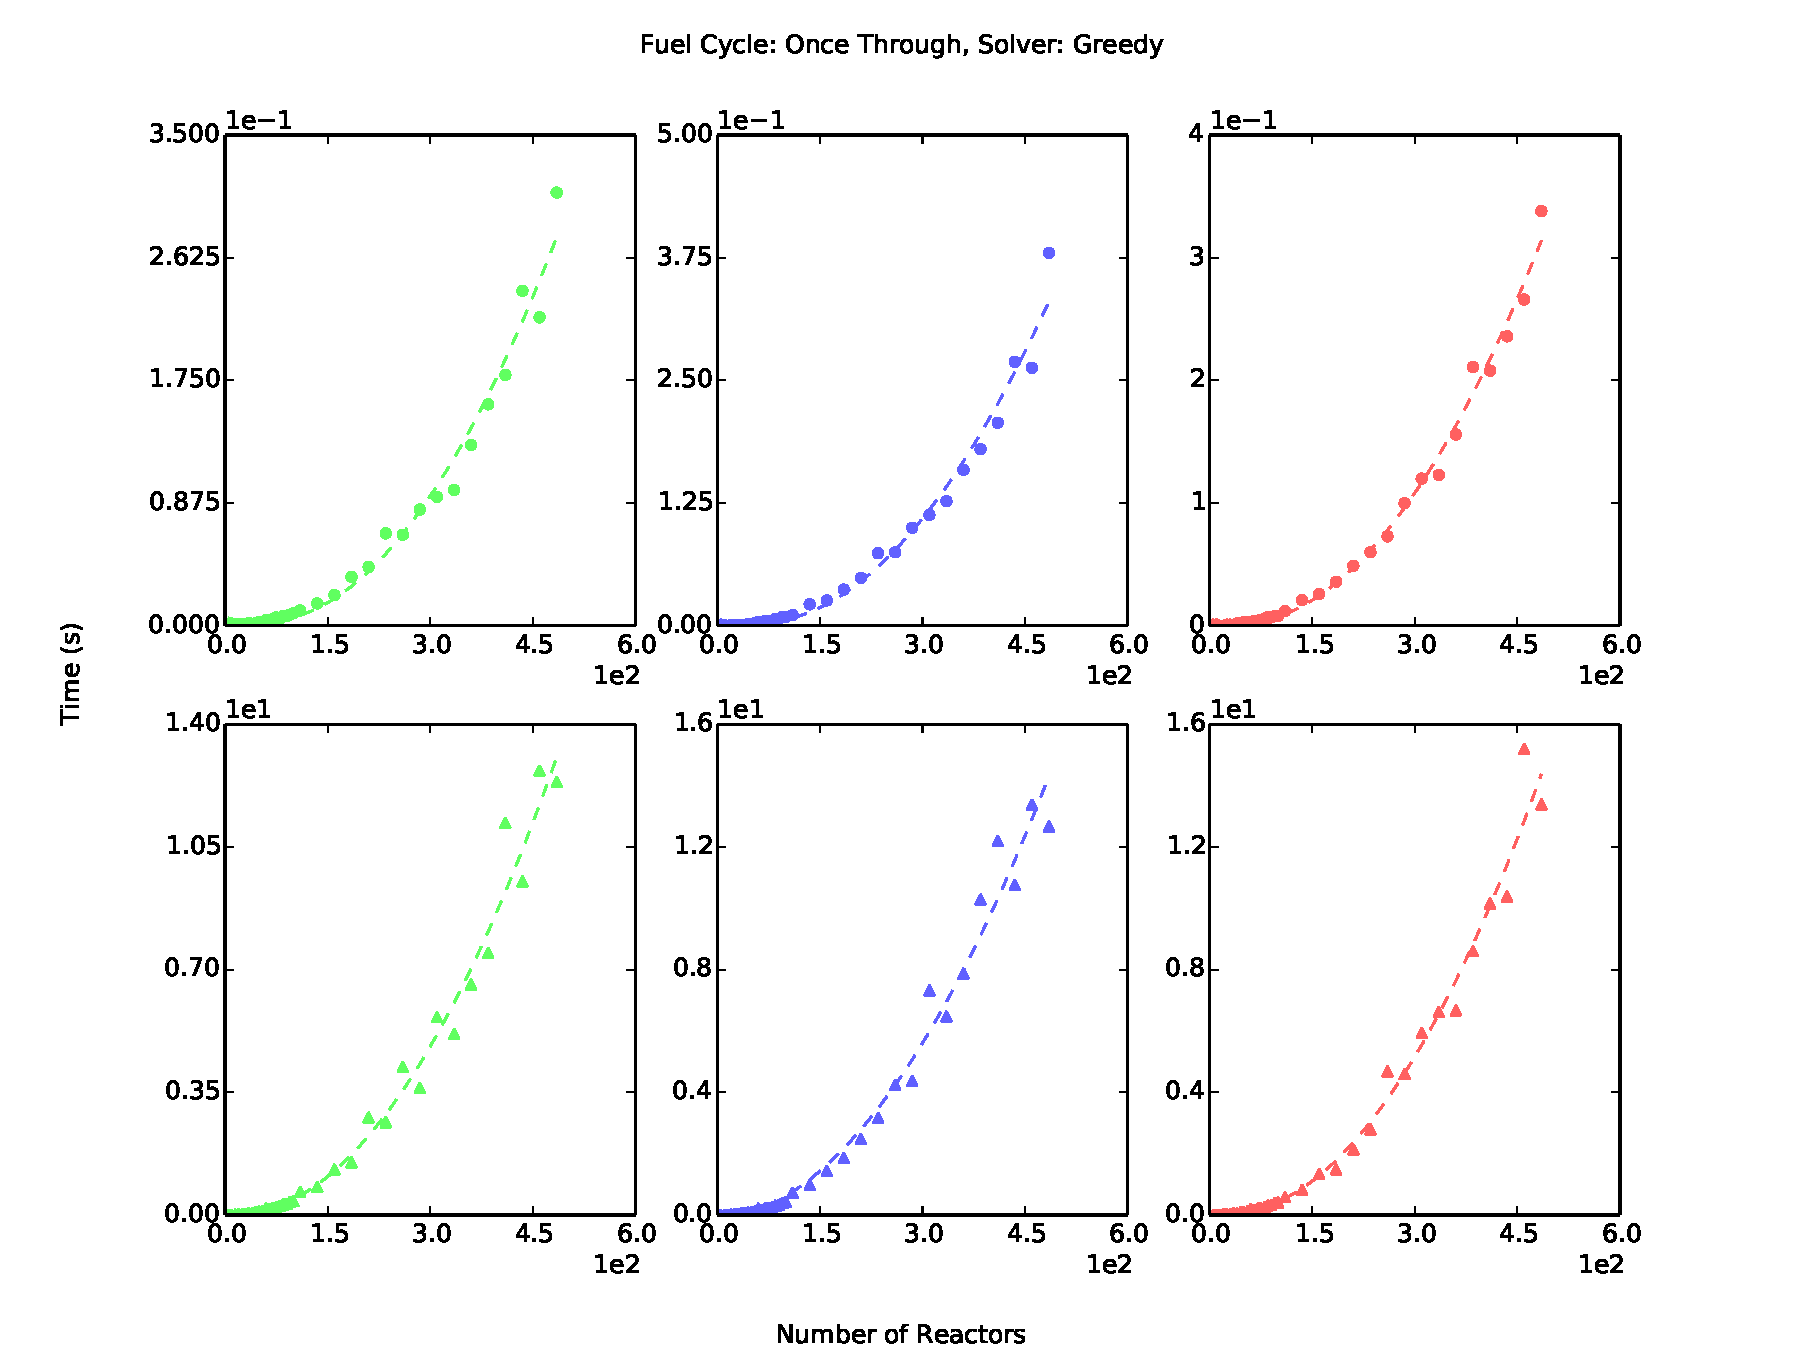
\includegraphics[width=.7\textwidth]{base_front_n_rxtr_time_fc0_solvergreedy.pdf}
    \caption[]{
      \label{fig:base_front_n_rxtr_time_fc0_solvergreedy}
      Greedy Solver results for the OT fuel cycle as the number of reactors
      increases.  }
  \end{center}
\end{figure}

\begin{figure}[h!]
  \begin{center}
    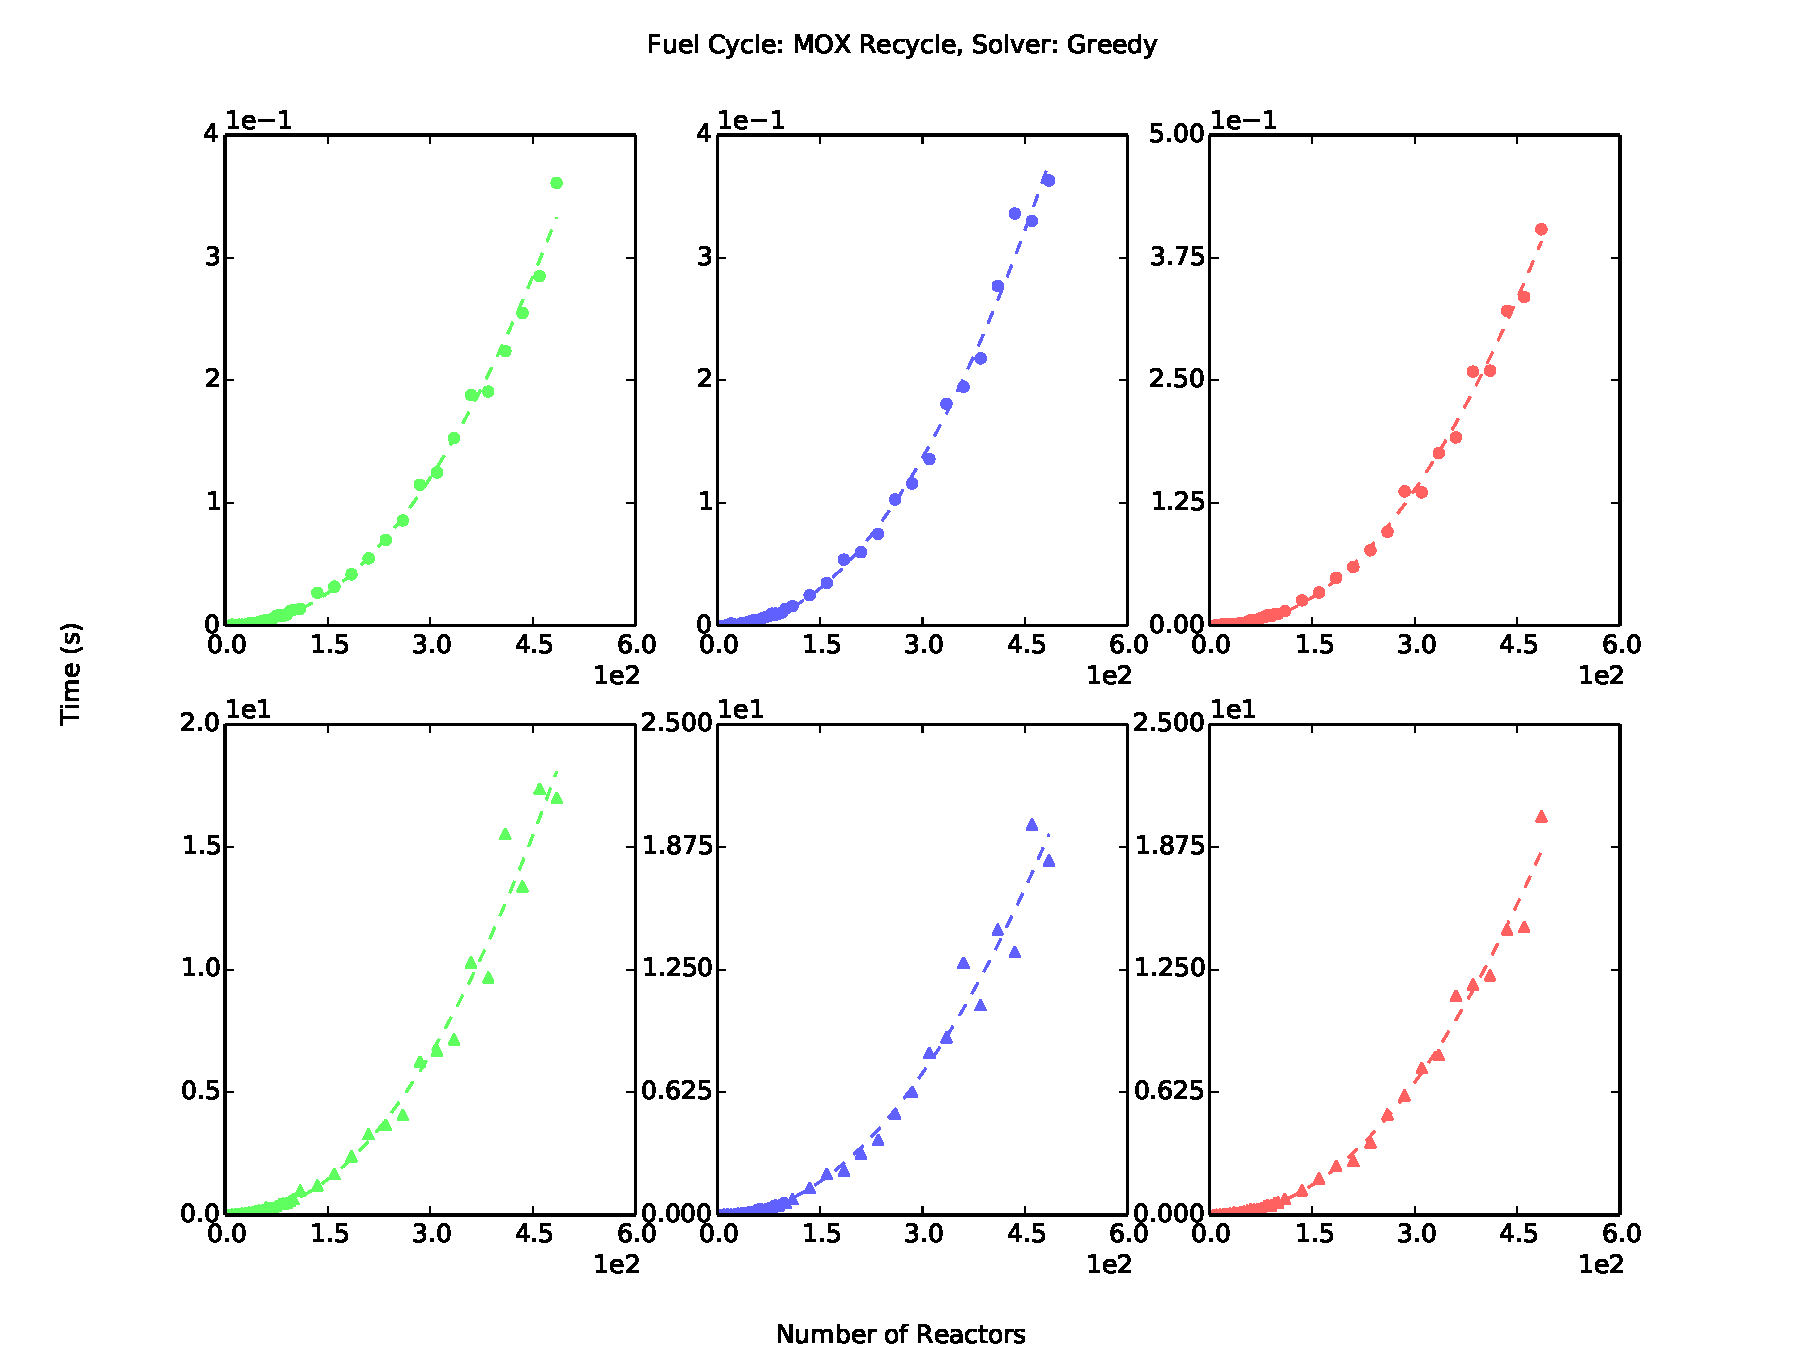
\includegraphics[width=.7\textwidth]{base_front_n_rxtr_time_fc1_solvergreedy.pdf}
    \caption[]{
      \label{fig:base_front_n_rxtr_time_fc1_solvergreedy}
      Greedy Solver results for the MOX fuel cycle as the number of reactors
      increases.
    }
  \end{center}
\end{figure}

\begin{figure}[h!]
  \begin{center}
    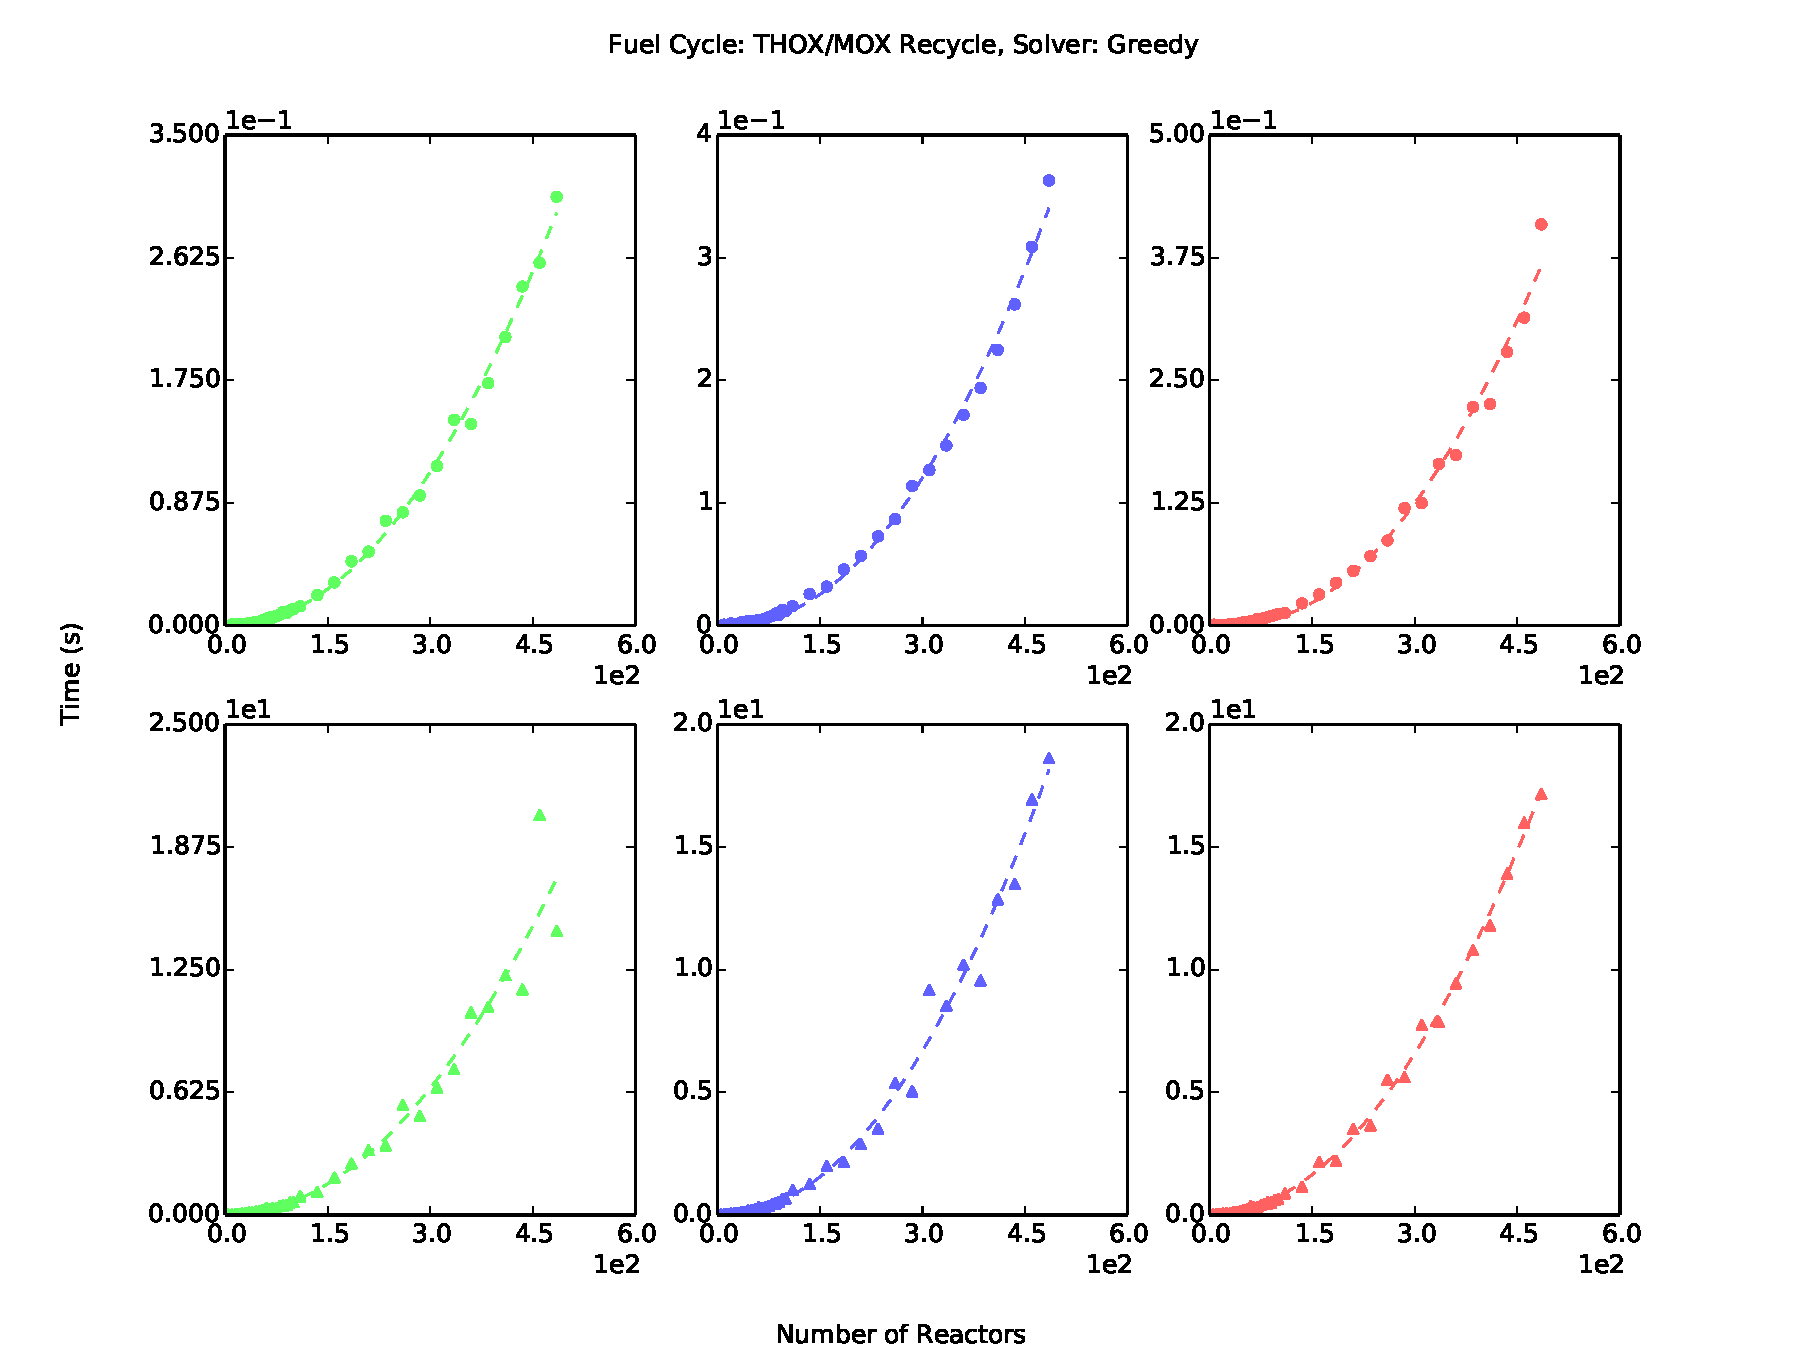
\includegraphics[width=.7\textwidth]{base_front_n_rxtr_time_fc2_solvergreedy.pdf}
    \caption[]{
      \label{fig:base_front_n_rxtr_time_fc2_solvergreedy}
      Greedy Solver results for the ThOX fuel cycle as the number of reactors
      increases.
      }
  \end{center}
\end{figure}

As was shown previously, the number of arcs in a generated exchange is an
$\mathcal{O}(n^2)$ effect. \ref{fig:base_front_n_arcs_time_fc1_solvergreedy}
graphs the same solution populations shown previously for the MOX fuel cycle as
a function of the number of arcs in the system. Plotted alongside the data are
linear curve fits. As can be seen, solution times scale linearly with the number
of arcs in the system. These trends are consistent across all three modeled fuel
cycles.

\begin{figure}[h!]
  \begin{center}
    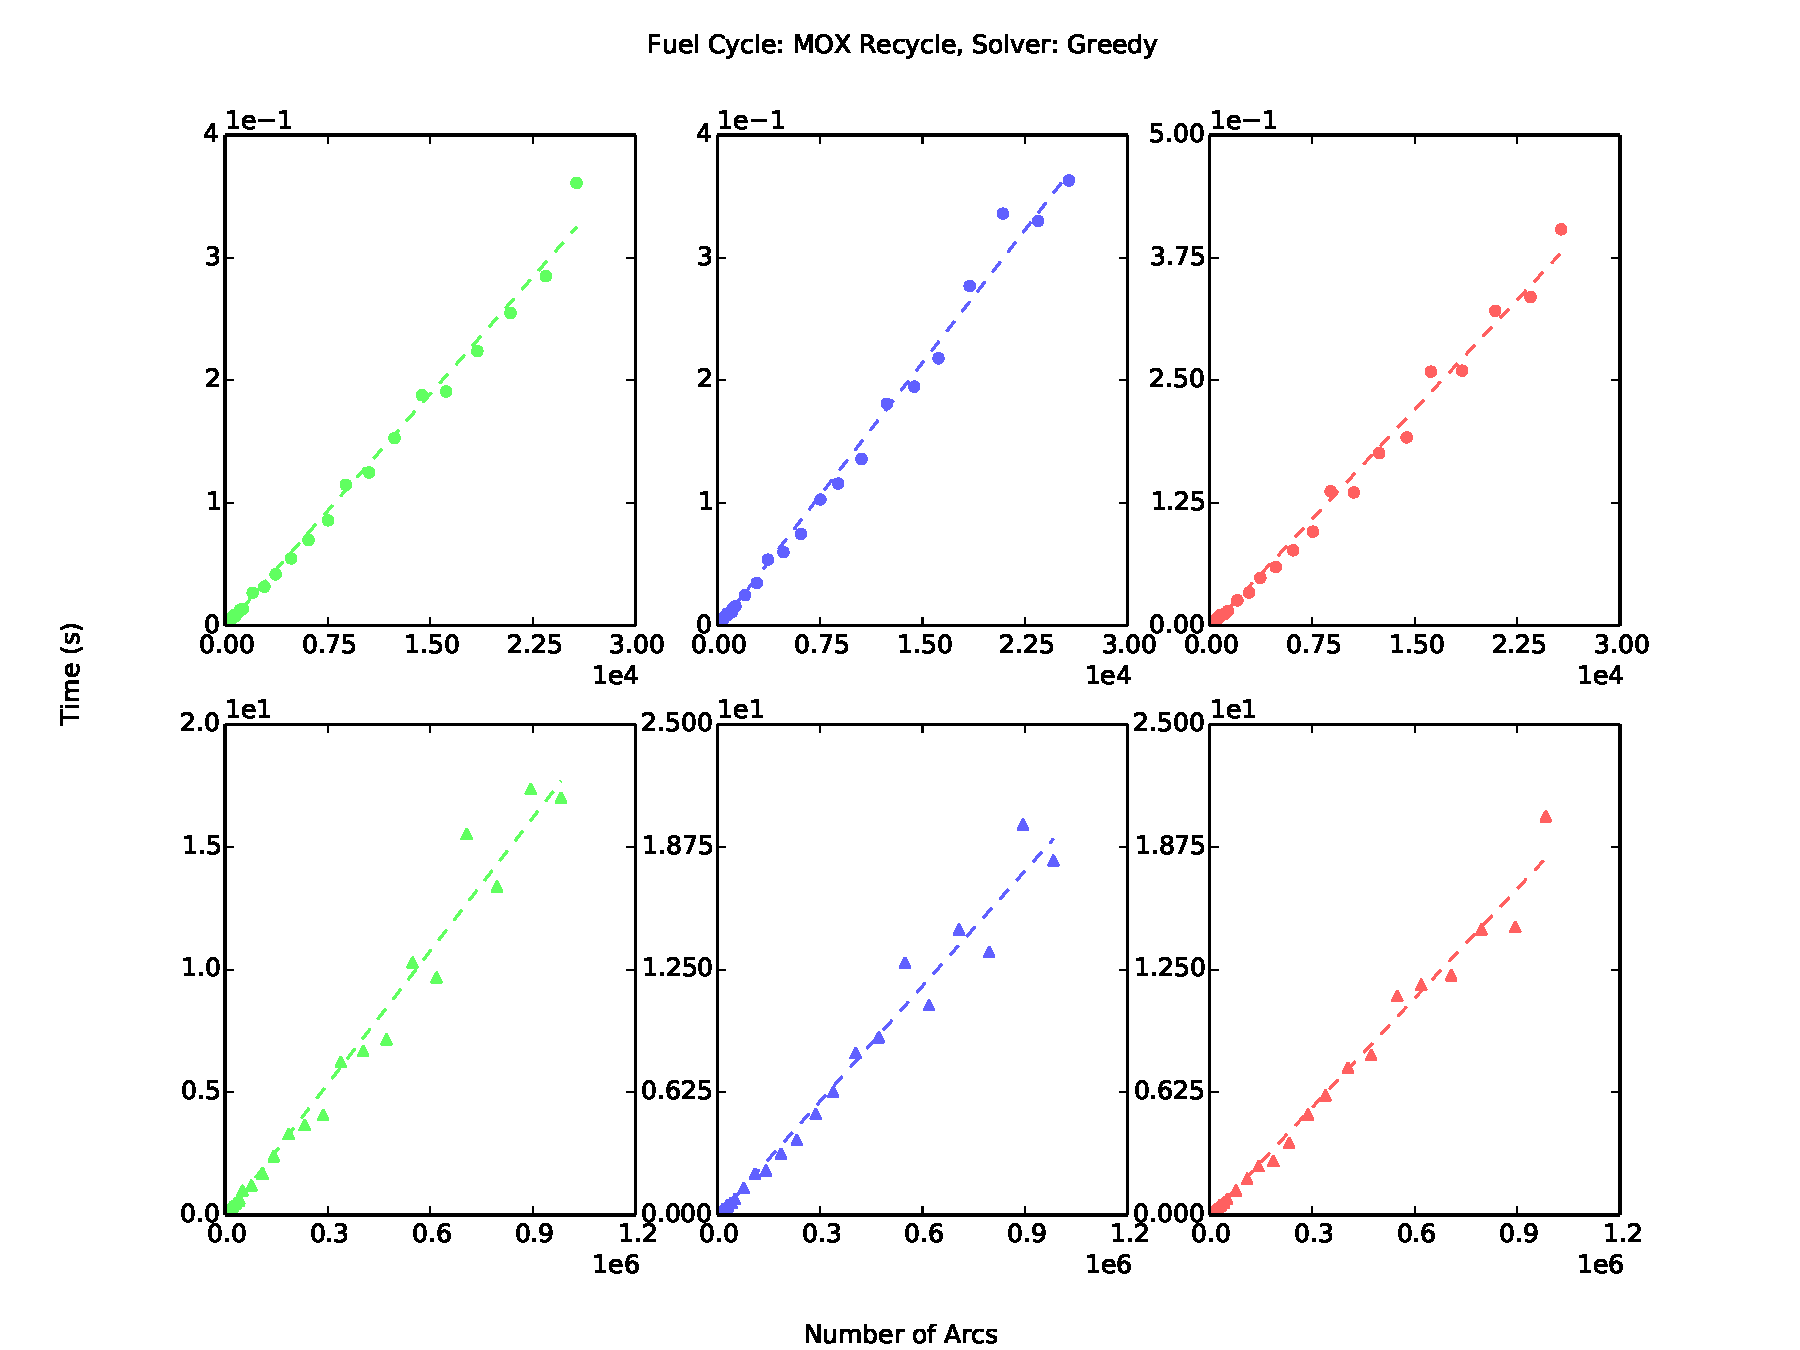
\includegraphics[width=.7\textwidth]{base_front_n_arcs_time_fc1_solvergreedy.pdf}
    \caption[]{
      \label{fig:base_front_n_arcs_time_fc1_solvergreedy}
      Greedy Solver results for the MOX fuel cycle as the number of arcs
      increases.      
    }
  \end{center}
\end{figure}

\paragraph{CLP Solver}

Interestingly, the CLP solver shows the same scaling behavior as the Greedy
Solver, and that behavior is also independent of fundamental parameter. The
number of arcs in the system drives the solution time scaling, as can be seen in
\Cref{fig:base_front_n_arcs_time_fc0_solverclp,fig:base_front_n_arcs_time_fc1_solverclp,fig:base_front_n_arcs_time_fc2_solverclp}.

\begin{figure}[h!]
  \begin{center}
    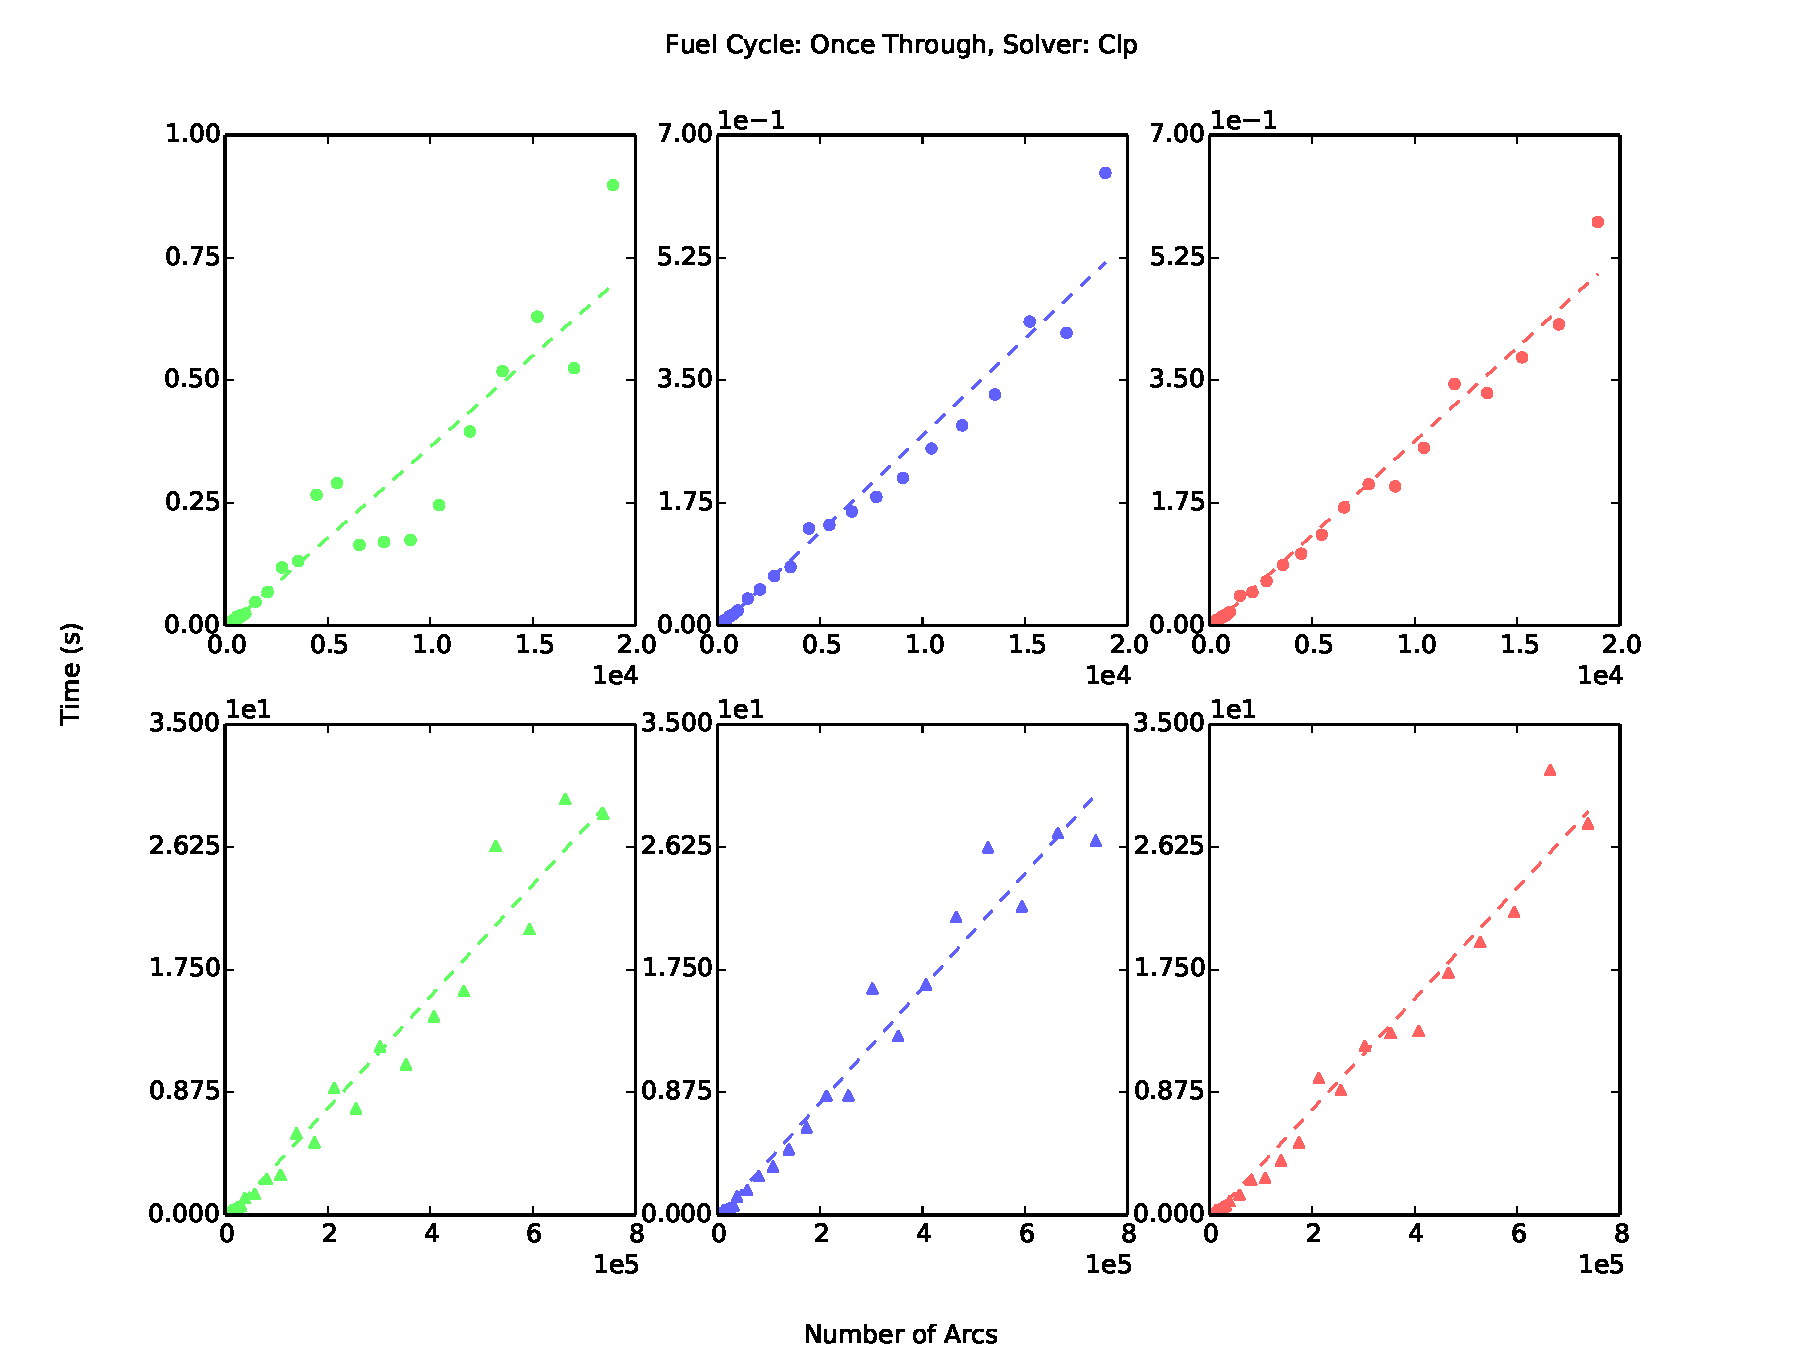
\includegraphics[width=.7\textwidth]{base_front_n_arcs_time_fc0_solverclp.pdf}
    \caption[]{
      \label{fig:base_front_n_arcs_time_fc0_solverclp}
      CLP Solver results for the OT fuel cycle as the number of arcs
      increases.
      }
  \end{center}
\end{figure}

\begin{figure}[h!]
  \begin{center}
    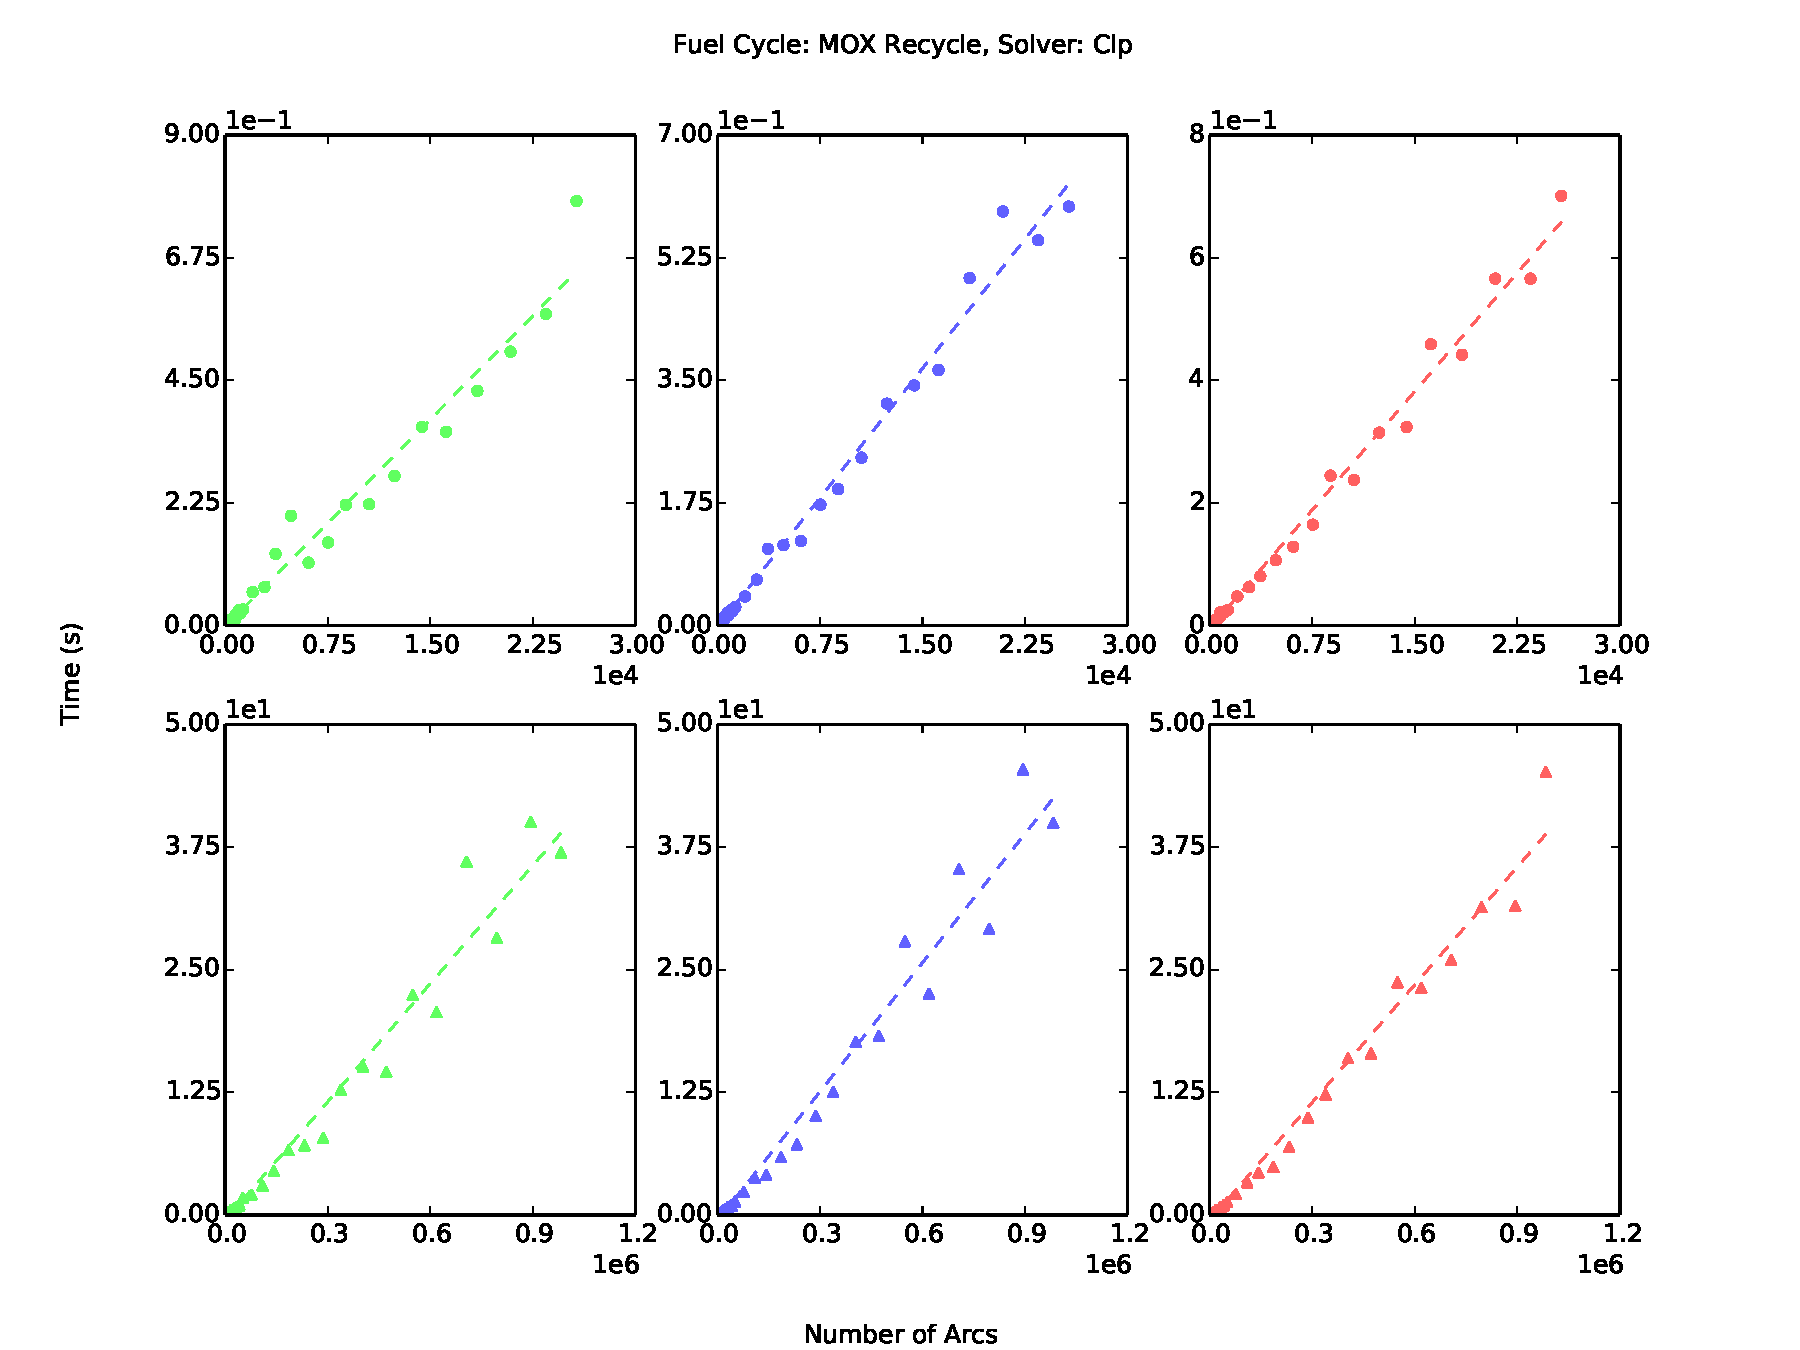
\includegraphics[width=.7\textwidth]{base_front_n_arcs_time_fc1_solverclp.pdf}
    \caption[]{
      \label{fig:base_front_n_arcs_time_fc1_solverclp}
      CLP Solver results for the MOX fuel cycle as the number of arcs
      increases.
      }
  \end{center}
\end{figure}

\begin{figure}[h!]
  \begin{center}
    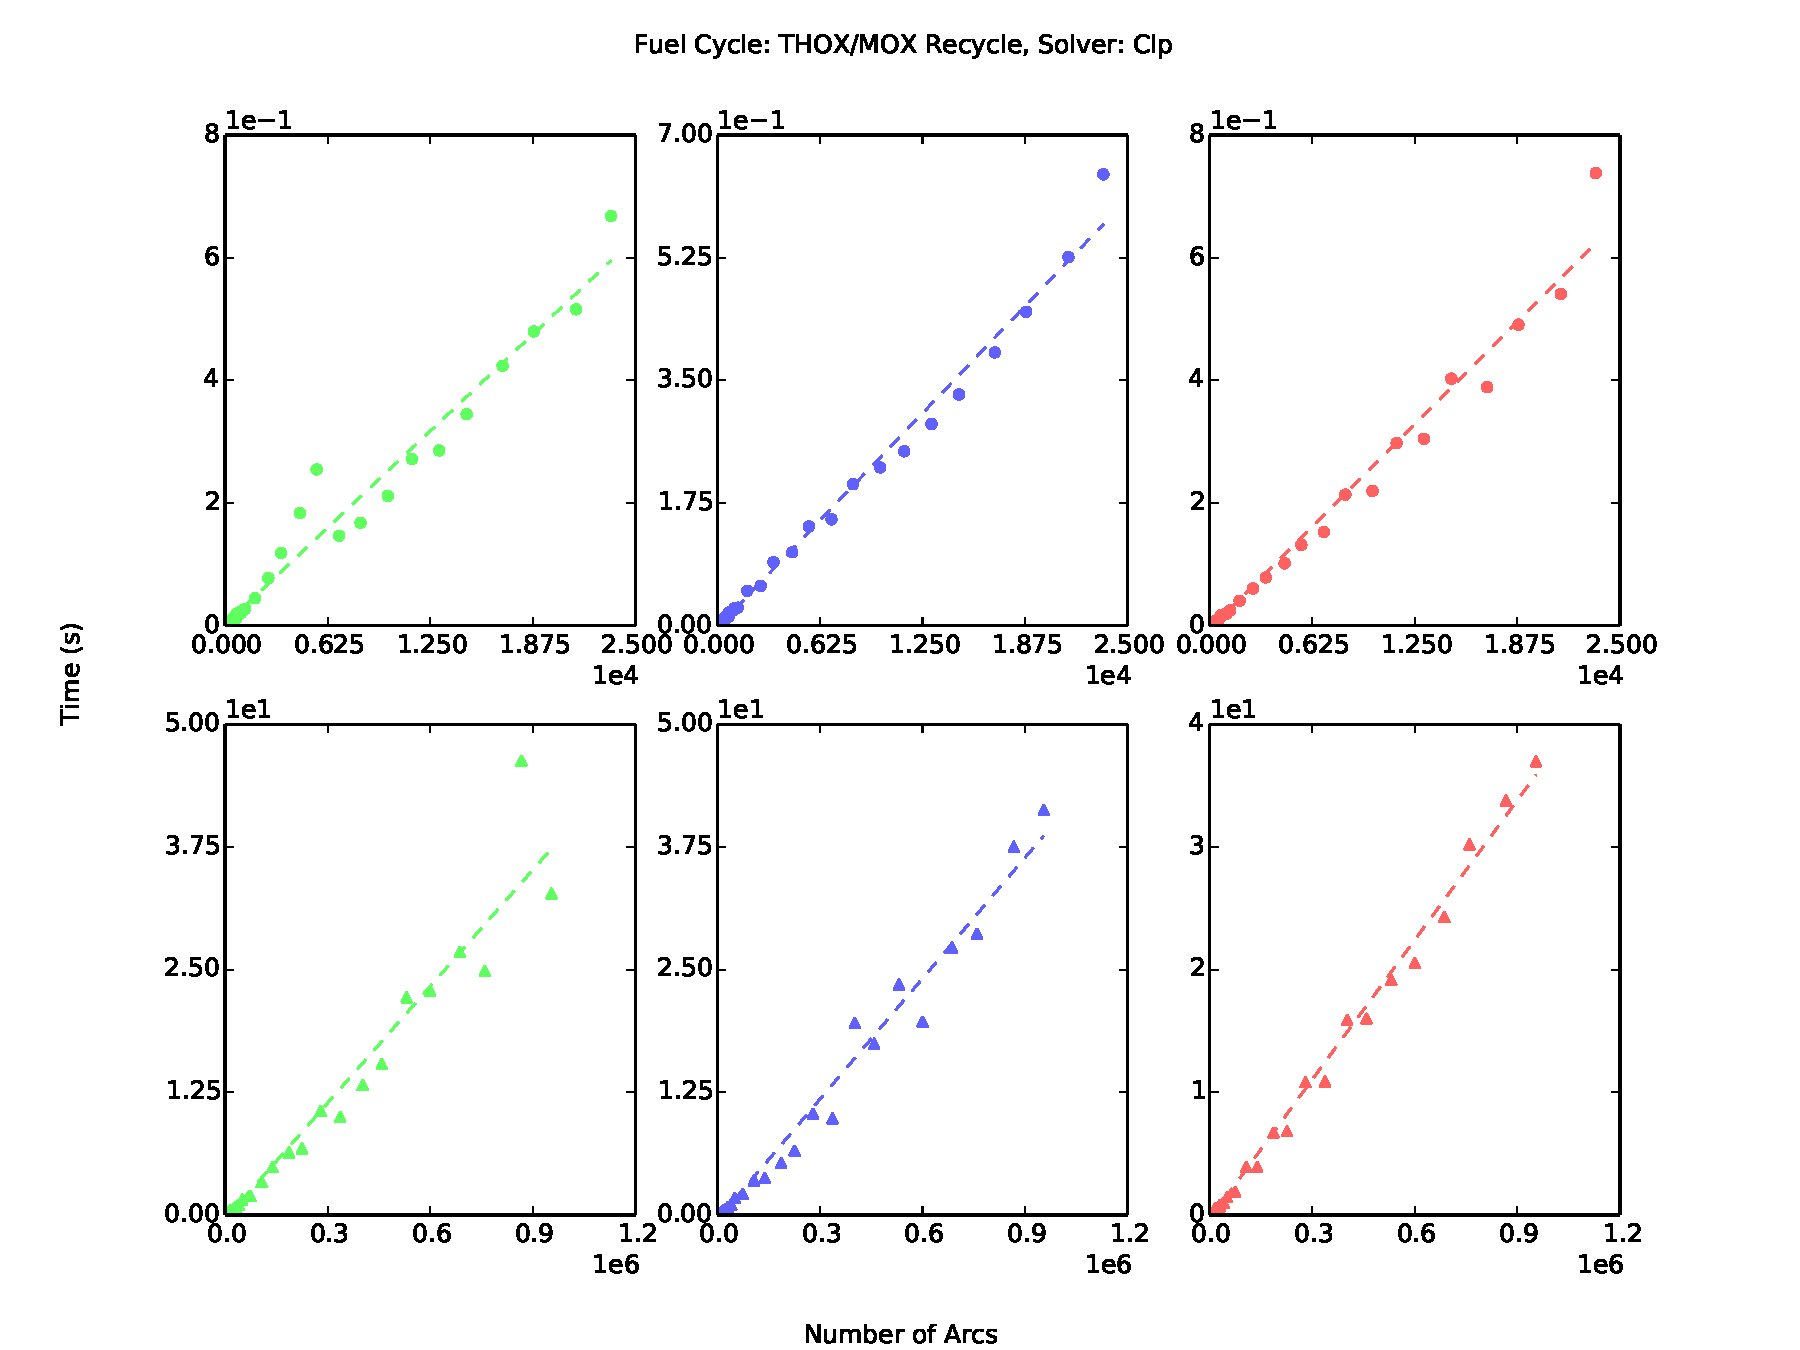
\includegraphics[width=.7\textwidth]{base_front_n_arcs_time_fc2_solverclp.pdf}
    \caption[]{
      \label{fig:base_front_n_arcs_time_fc2_solverclp}
      CLP Solver results for the ThOX fuel cycle as the number of arcs
      increases.
      }
  \end{center}
\end{figure}

\paragraph{CBC Solver}

The CBC solver is much more sporadic than either the CLP or Greedy solvers, as
is expected, for MILP optimization problems are NP-Hard. An artificial, 3-hour
time limit was provided for CBC-solved instances, and a 1\% ratio-gap
convergence criteria was applied. In each of the figures below, only instances
reaching convergence are displayed in order to attempt to ascertain any related
trends. \Cref{fig:base_front_n_rxtr_time_fc0_solvercbc,fig:base_front_n_rxtr_time_fc1_solvercbc,fig:base_front_n_rxtr_time_fc2_solvercbc}
show timing results as a function of the number of reactors in the
system. \Cref{fig:base_front_n_arcs_time_fc0_solvercbc,fig:base_front_n_arcs_time_fc1_solvercbc,fig:base_front_n_arcs_time_fc2_solvercbc}
show timing results as a function of the number of arcs in the system. Note that
in each case below, a log-lin graph is used.

\begin{figure}[h!]
  \begin{center}
    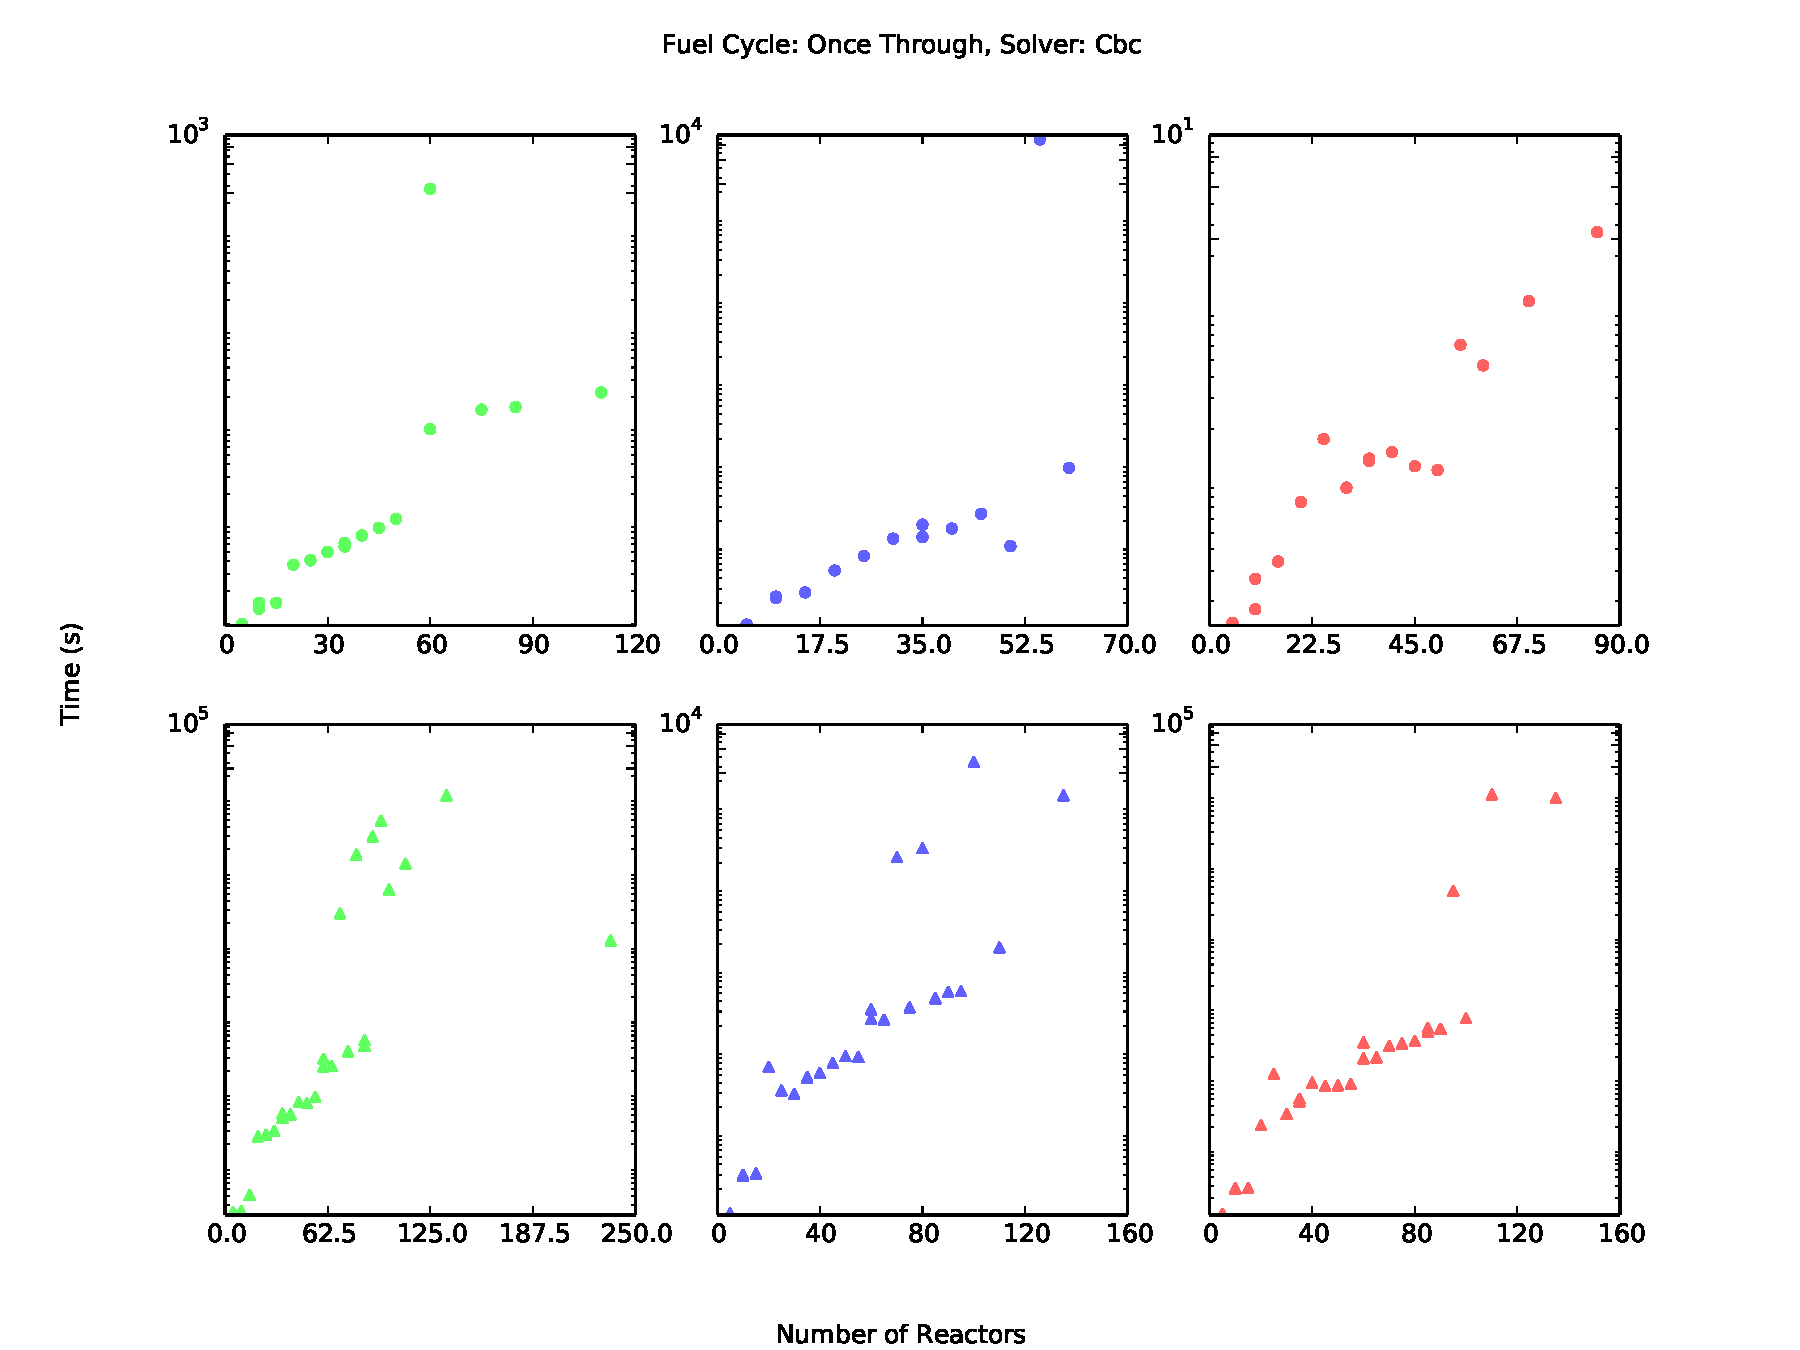
\includegraphics[width=.7\textwidth]{base_front_n_rxtr_time_fc0_solvercbc.pdf}
    \caption[]{
      \label{fig:base_front_n_rxtr_time_fc0_solvercbc}
      CBC Solver results for the OT fuel cycle as the number of reactors
      increases.
      }
  \end{center}
\end{figure}

\begin{figure}[h!]
  \begin{center}
    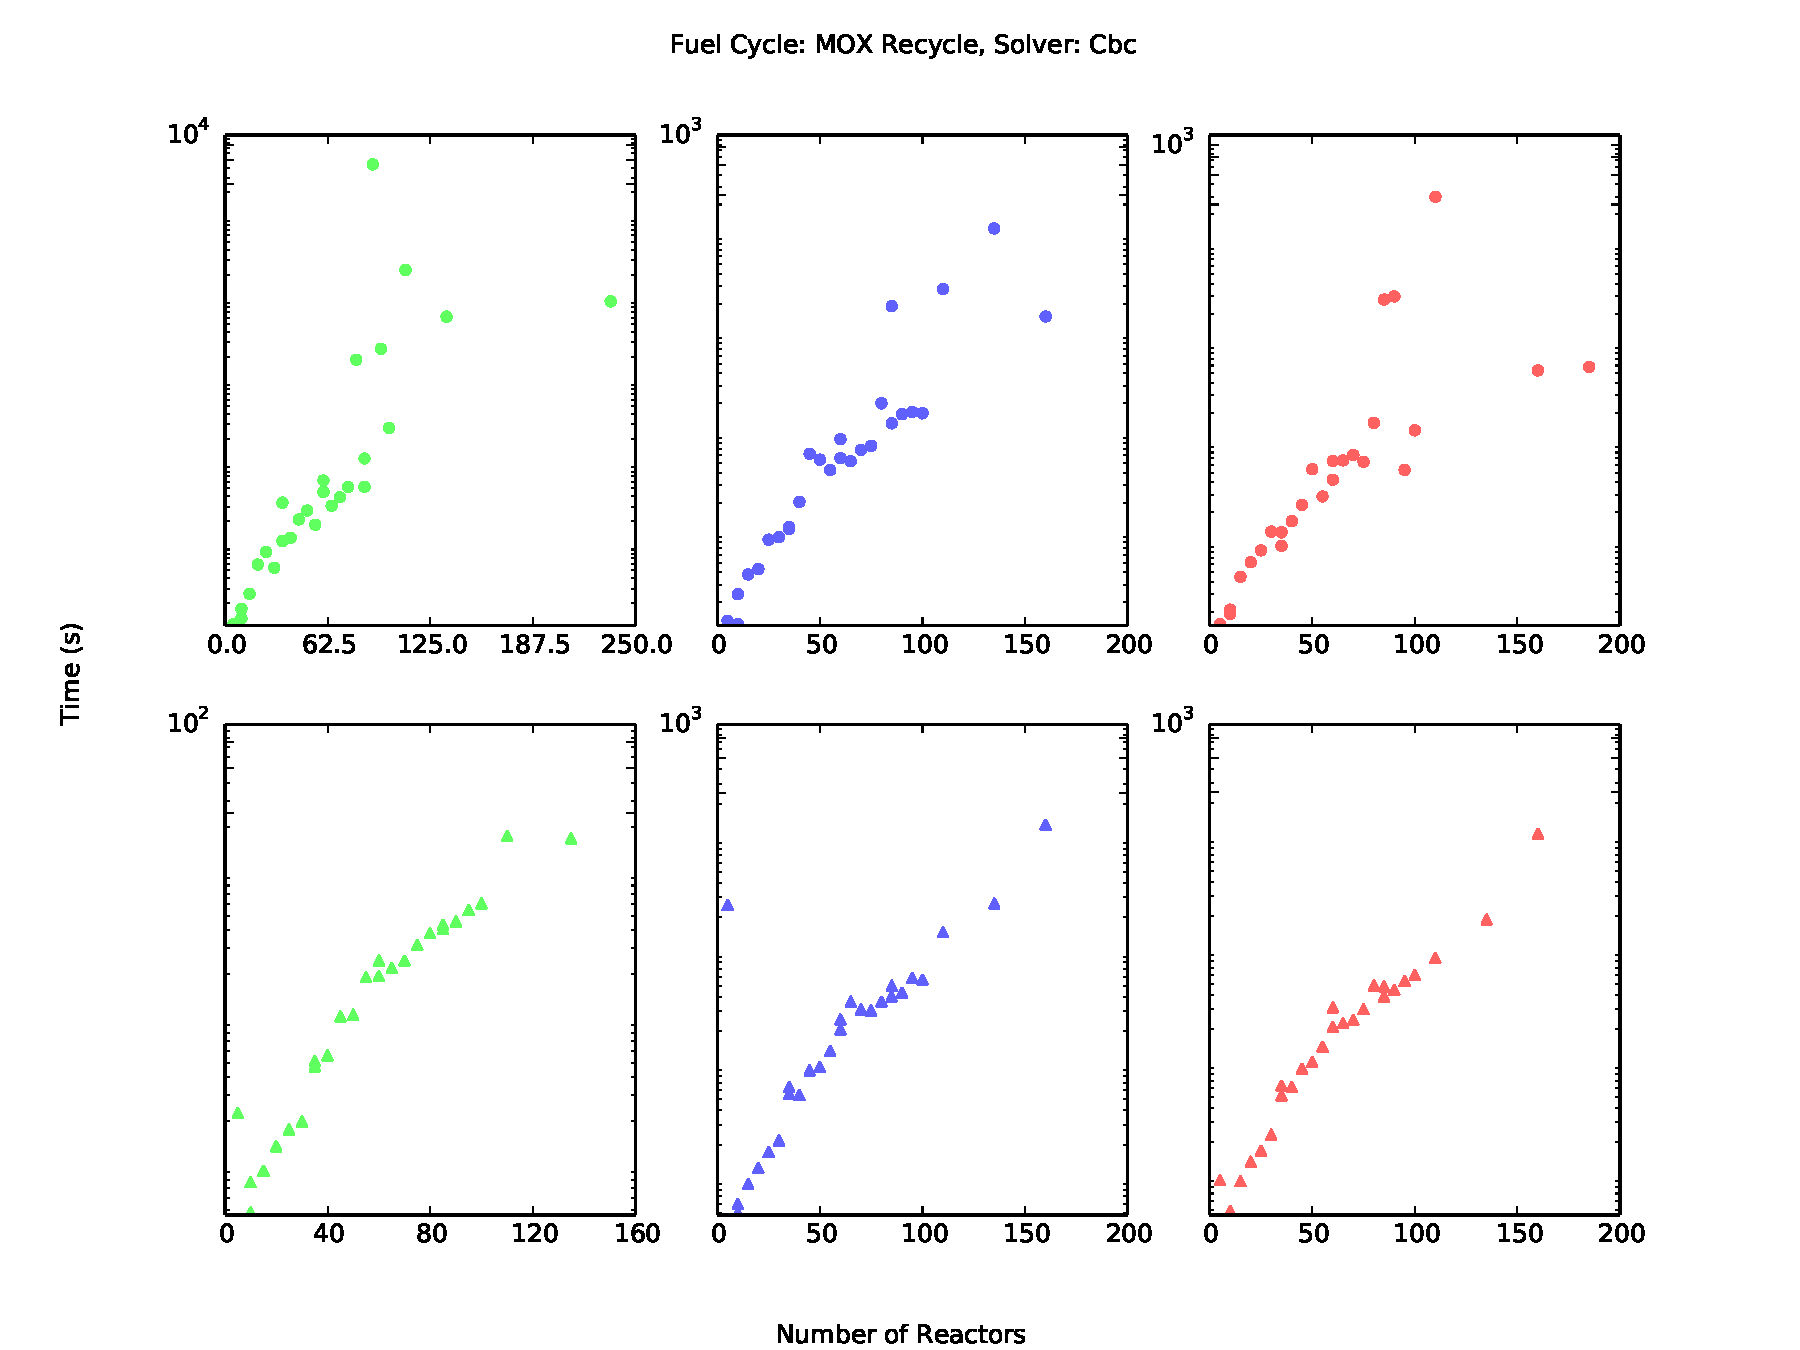
\includegraphics[width=.7\textwidth]{base_front_n_rxtr_time_fc1_solvercbc.pdf}
    \caption[]{
      \label{fig:base_front_n_rxtr_time_fc1_solvercbc}
      CBC Solver results for the MOX fuel cycle as the number of reactors
      increases.
      }
  \end{center}
\end{figure}

\begin{figure}[h!]
  \begin{center}
    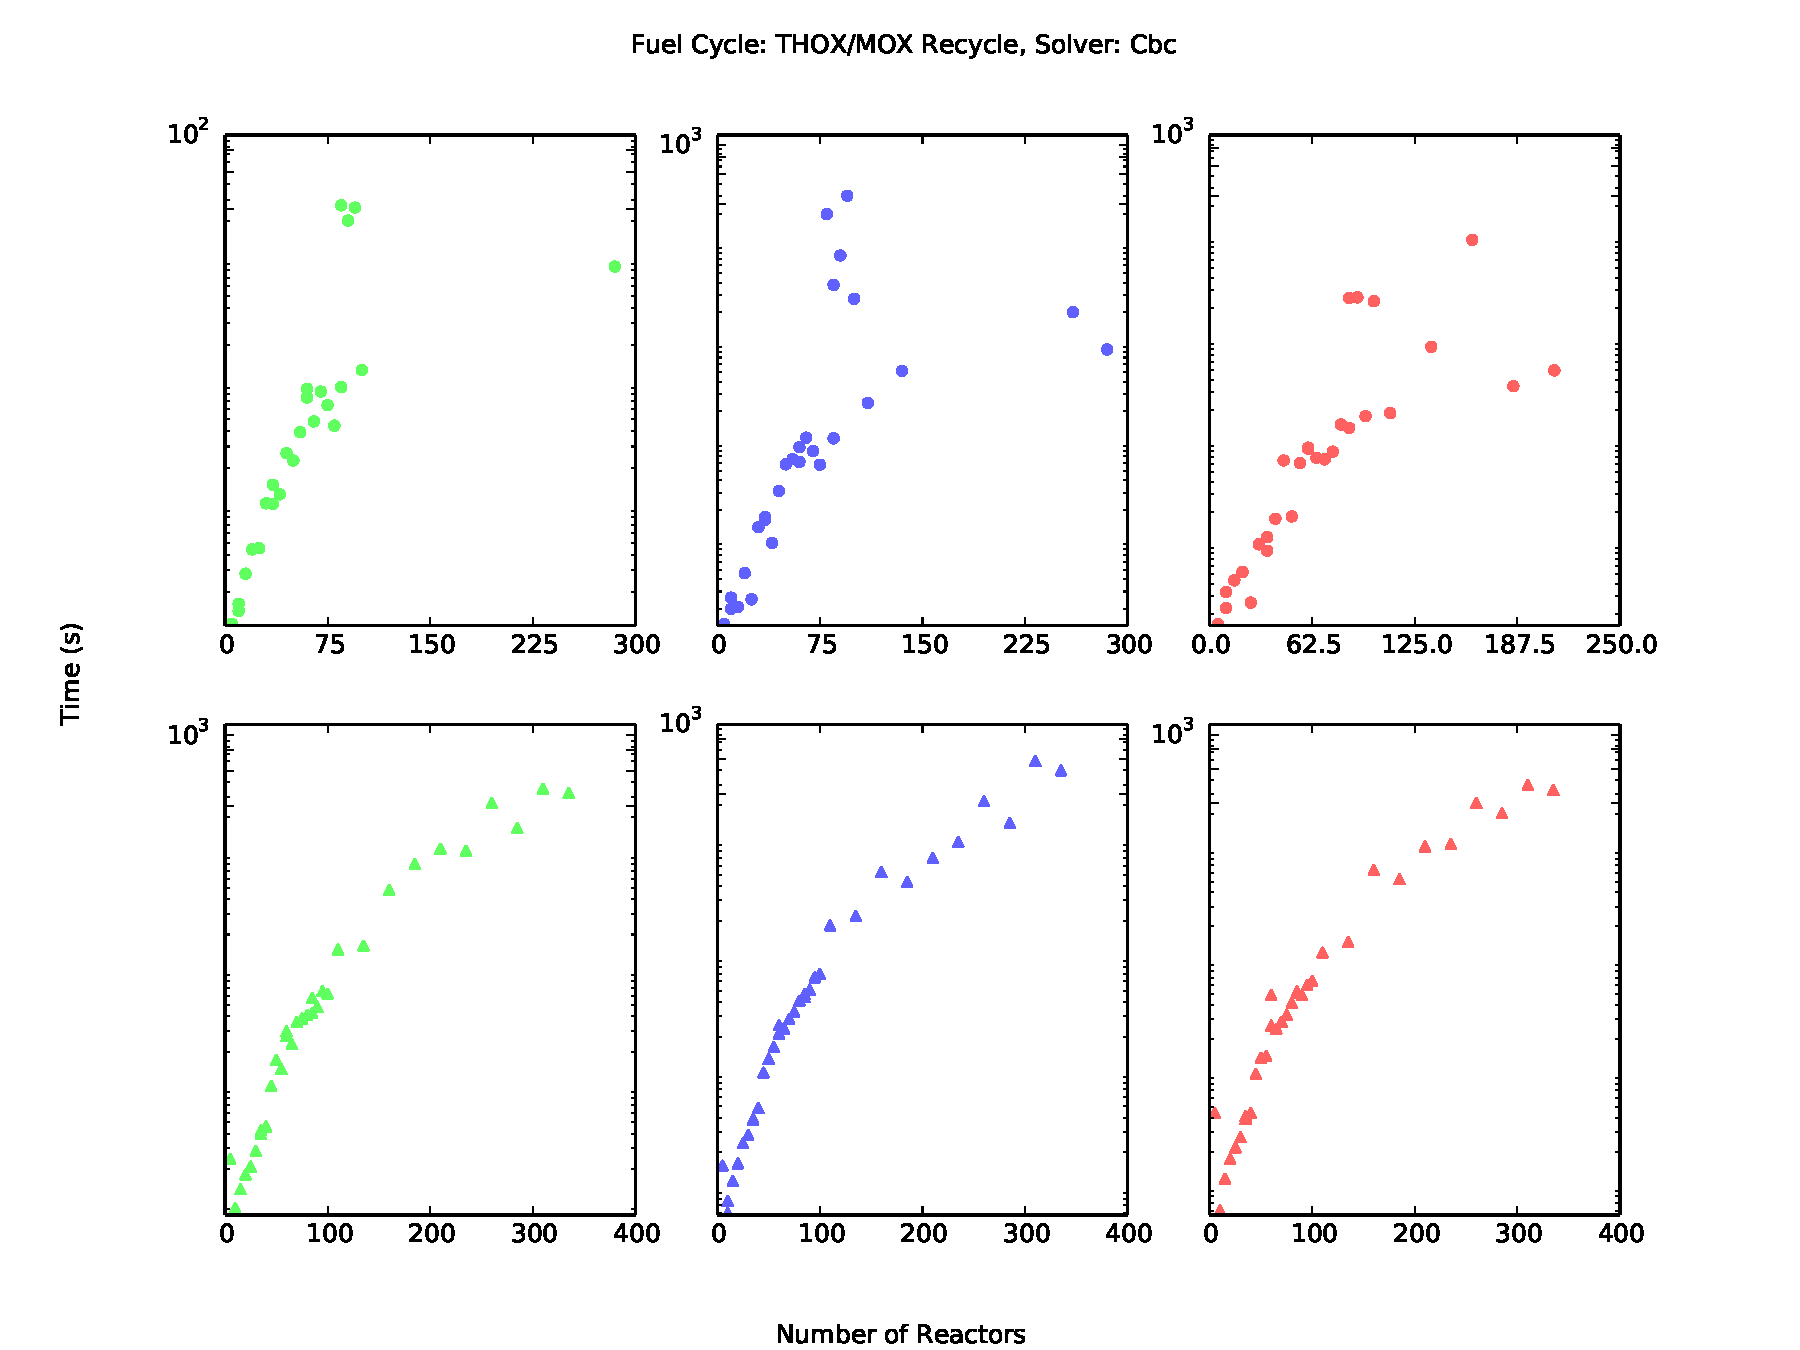
\includegraphics[width=.7\textwidth]{base_front_n_rxtr_time_fc2_solvercbc.pdf}
    \caption[]{
      \label{fig:base_front_n_rxtr_time_fc2_solvercbc}
      CBC Solver results for the ThOX fuel cycle as the number of reactors
      increases.
      }
  \end{center}
\end{figure}

\begin{figure}[h!]
  \begin{center}
    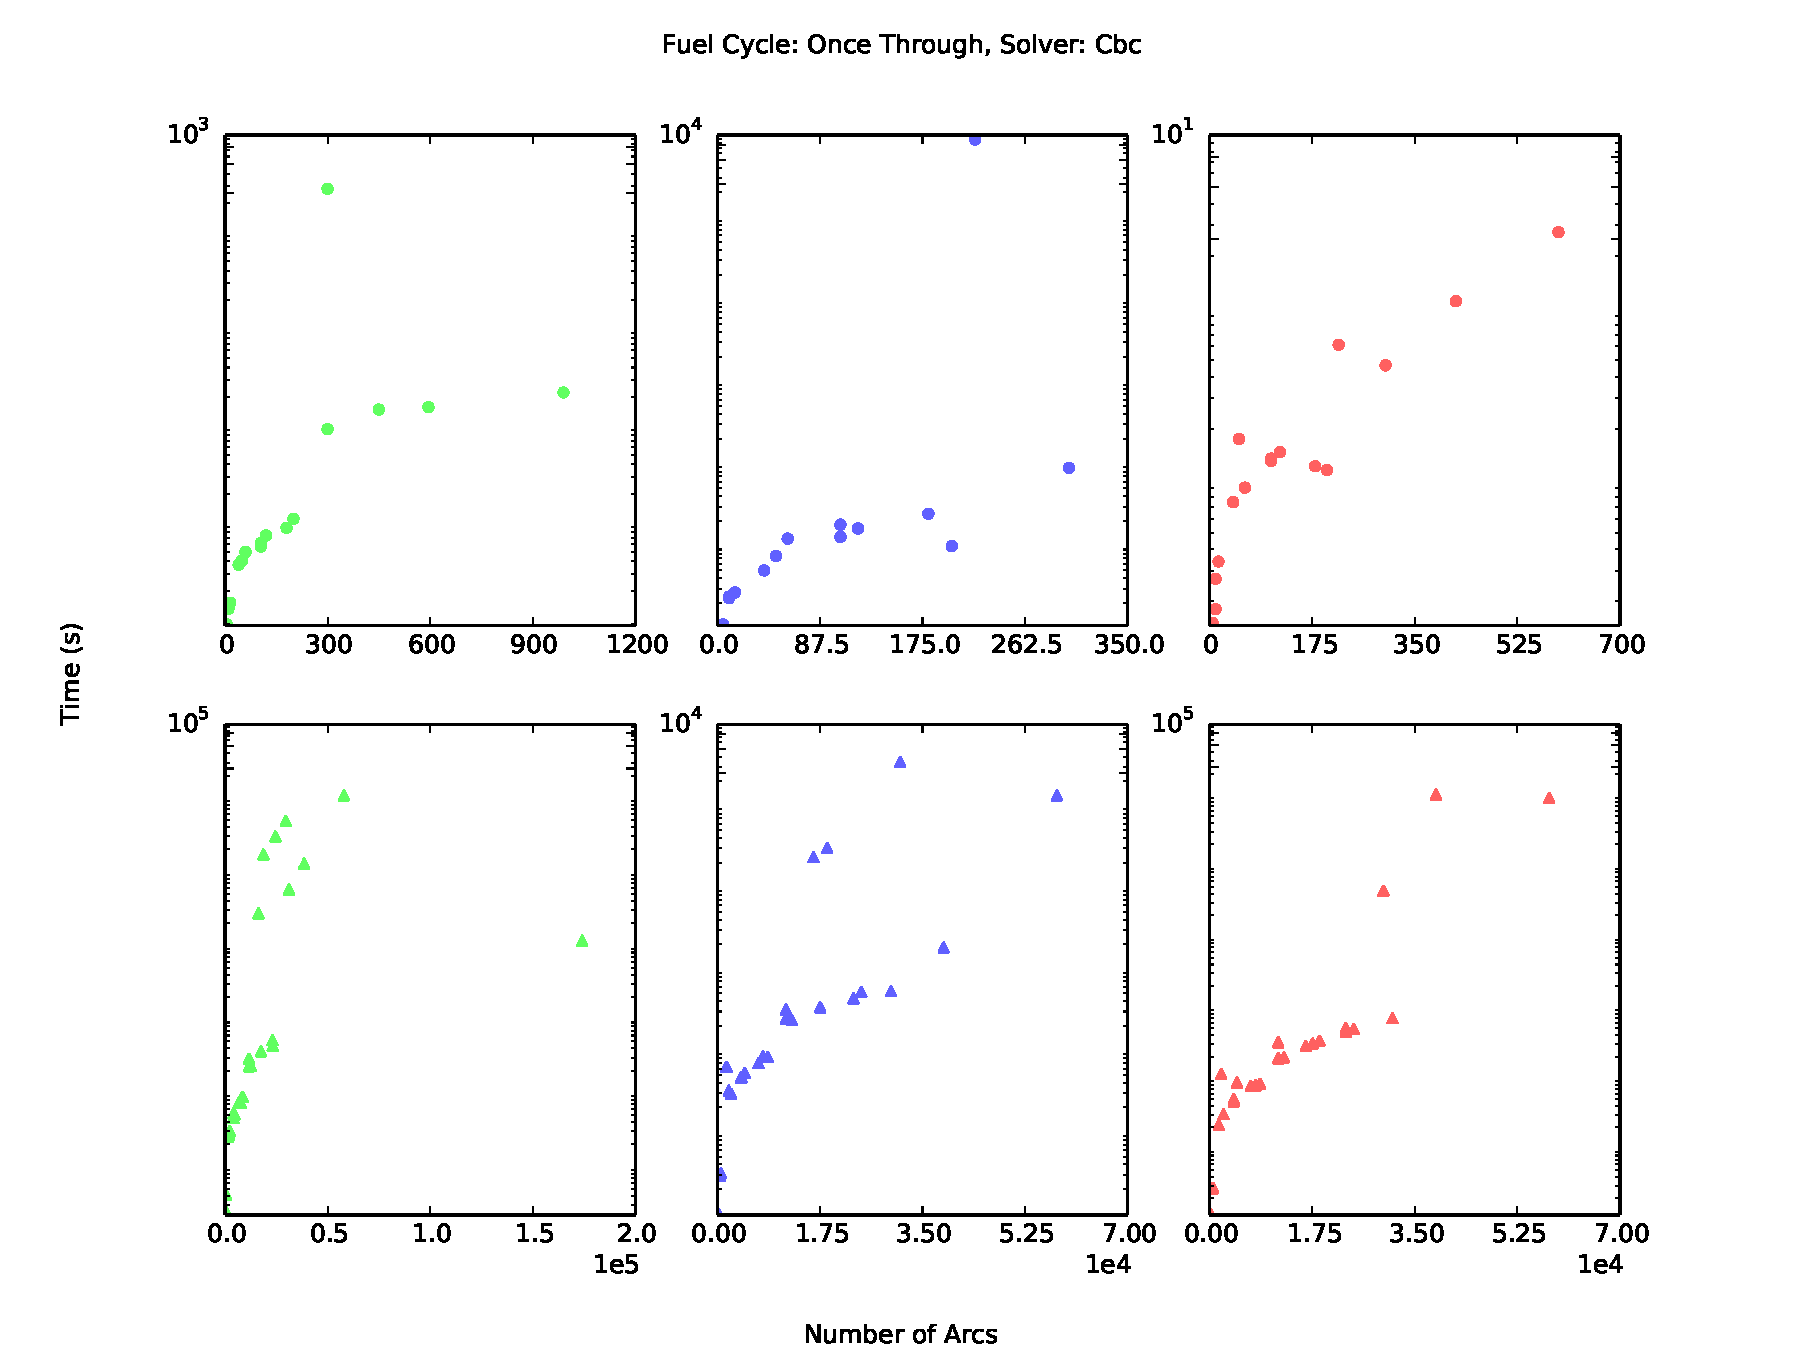
\includegraphics[width=.7\textwidth]{base_front_n_arcs_time_fc0_solvercbc.pdf}
    \caption[]{
      \label{fig:base_front_n_arcs_time_fc0_solvercbc}
      CBC Solver results for the OT fuel cycle as the number of arcs
      increases.
      }
  \end{center}
\end{figure}

\begin{figure}[h!]
  \begin{center}
    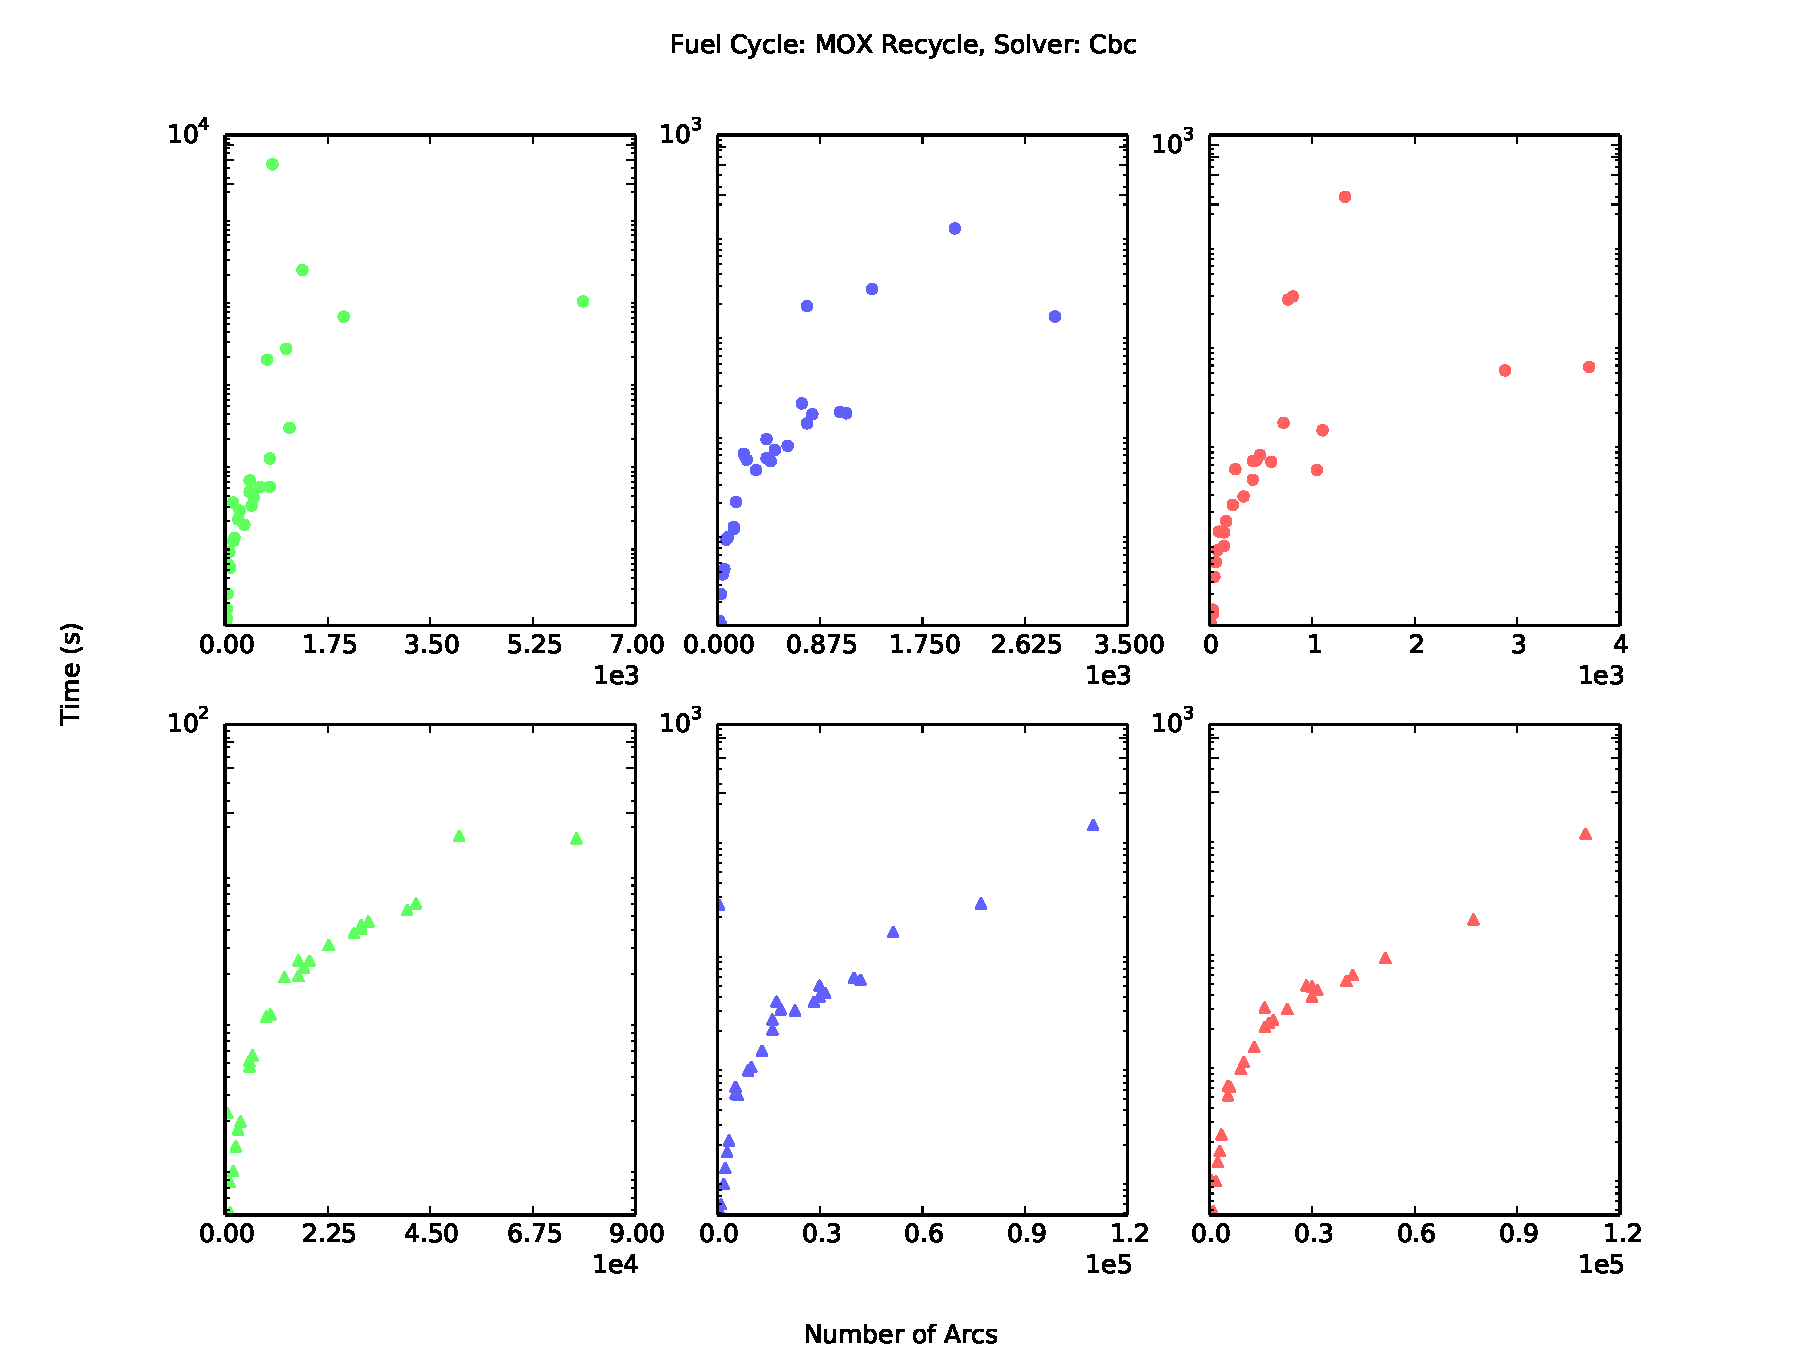
\includegraphics[width=.7\textwidth]{base_front_n_arcs_time_fc1_solvercbc.pdf}
    \caption[]{
      \label{fig:base_front_n_arcs_time_fc1_solvercbc}
      CBC Solver results for the MOX fuel cycle as the number of arcs
      increases.
      }
  \end{center}
\end{figure}

\begin{figure}[h!]
  \begin{center}
    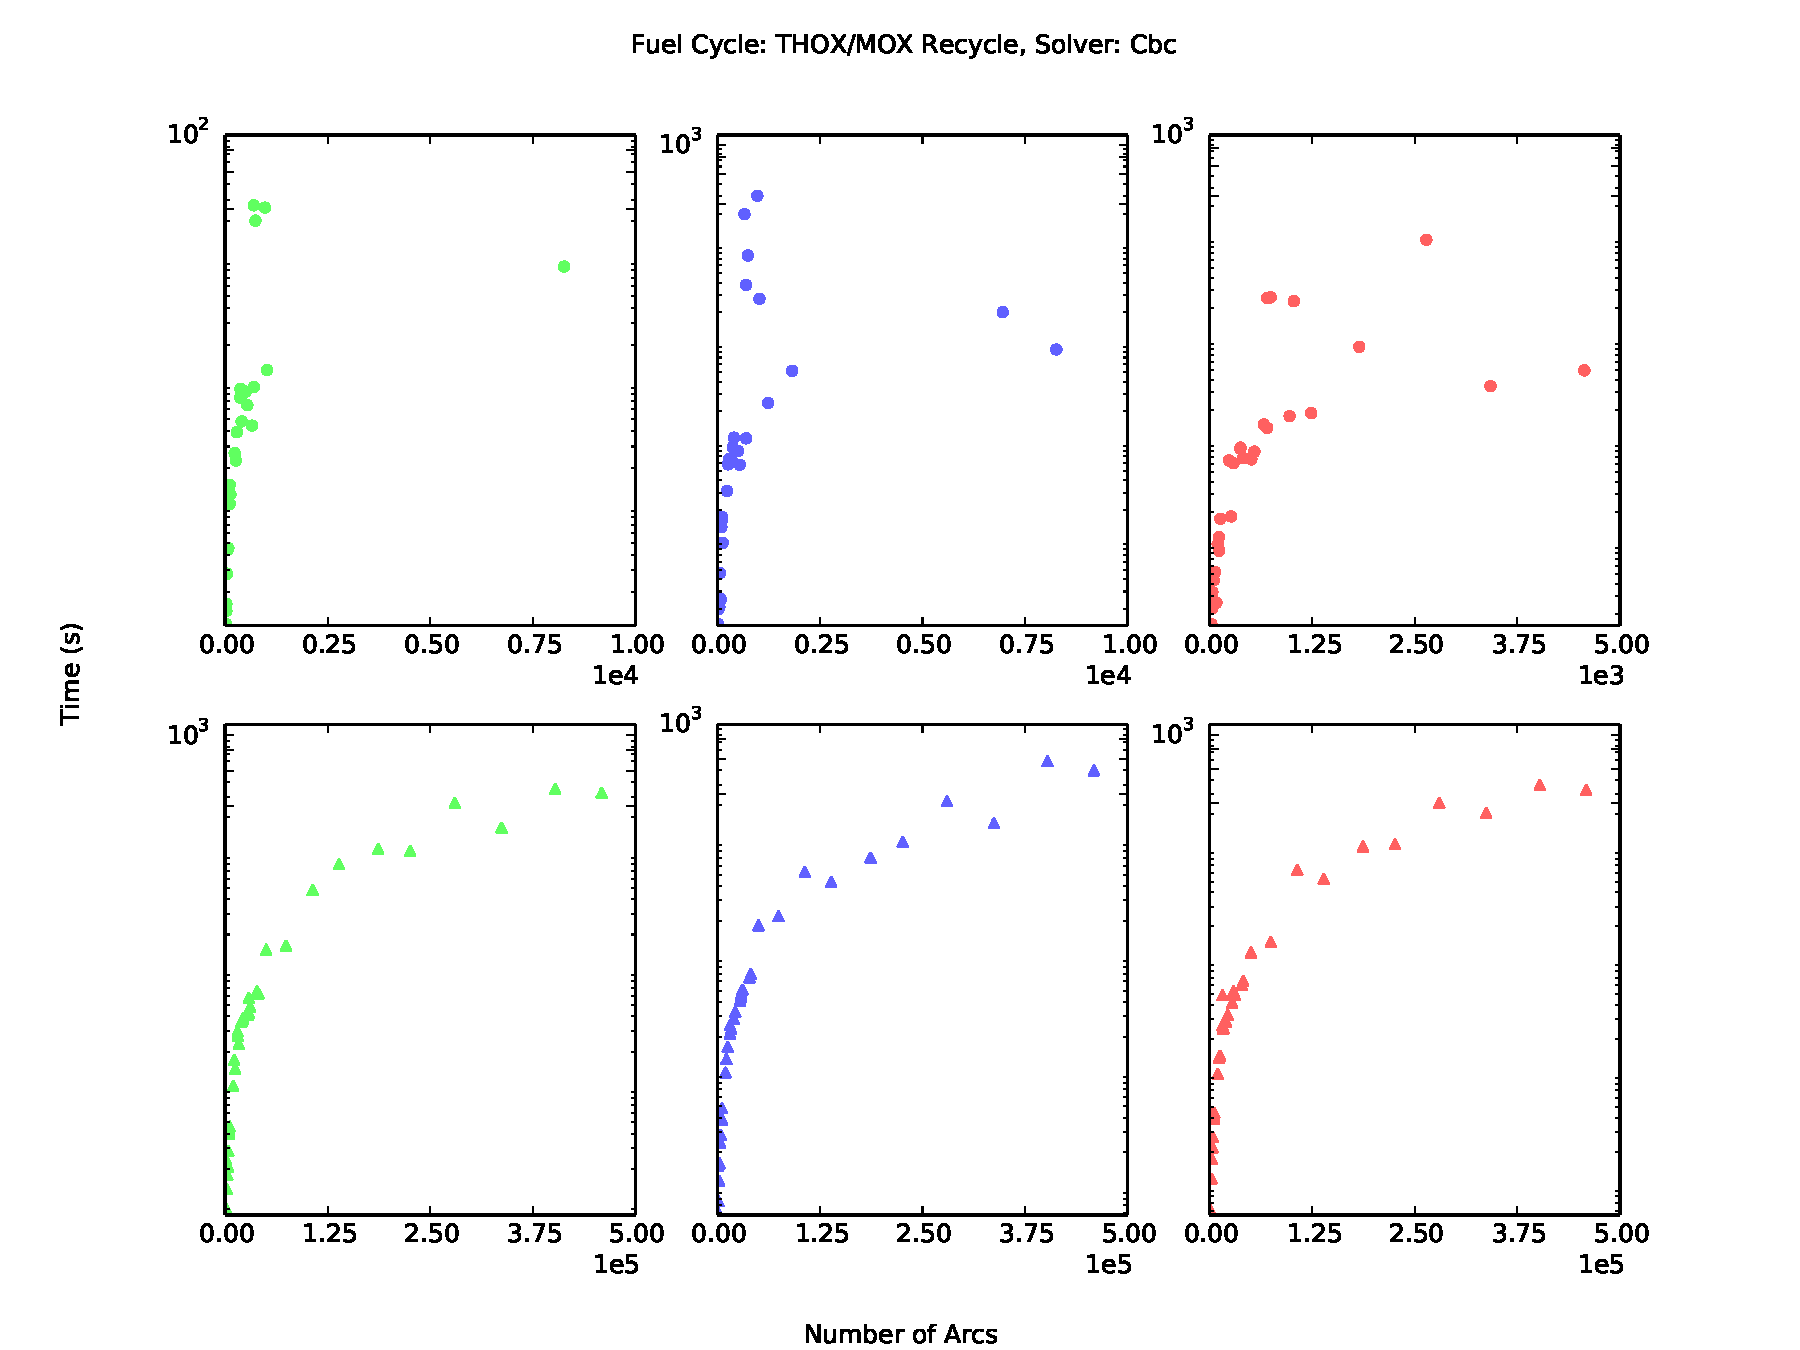
\includegraphics[width=.7\textwidth]{base_front_n_arcs_time_fc2_solvercbc.pdf}
    \caption[]{
      \label{fig:base_front_n_arcs_time_fc2_solvercbc}
      CBC Solver results for the ThOX fuel cycle as the number of arcs
      increases.
      }
  \end{center}
\end{figure}

Immediately obvious, and slightly counter intuitive, is that the population of
converged instances is larger for assembly-based exchanges rather than
batch-based exchanges, even though the number of variables in the problem is
much lower for batch-based exchanges. 

\TODO{More Explanation..}

%% \subsubsection{Instance Parameter Variation}
%% % Include large and small r_l_c

%% \paragraph{Location-to-Commodity Importance Ratio}

%% \paragraph{Thermal and Fast-Reactor Populations}

%% \paragraph{Inventory vs. Processing Constraints}

\subsubsection{Convergence Criteria}

The CBC solver is highly tuneable. Perhaps the most critical tuneable criteria
affecting the balance between solution quality and solution time is the
convergence criteria. It is not clear to what degree solution quality will
matter for users of Cyclus. Accordingly, a short exploratory experiment was
conducted to examine to what degree convergence criteria affects solution time.

CBC uses either an absolute or relative upper and lower-bound gap tolerance as
possible convergence criteria. This experiment uses the relative gap, termed
\textit{ratio gap} in CBC parlance. For each of the 18 combinations of
fundamental parameters, 10 instances of exchanges were executed, spanning a
reactor population range of 10 to 500. Figure \ref{fig:hist_front_rxtr_0}
displays the results for runs with reactors trading full batches for ratio gap
values of 0.1, 1, and 10\%. Figure \ref{fig:hist_front_rxtr_0} displays the
results for runs with reactors trading individual assemblies for ratio gap
values of 1 and 10\%.

\begin{figure}[h!]
  \begin{center}
    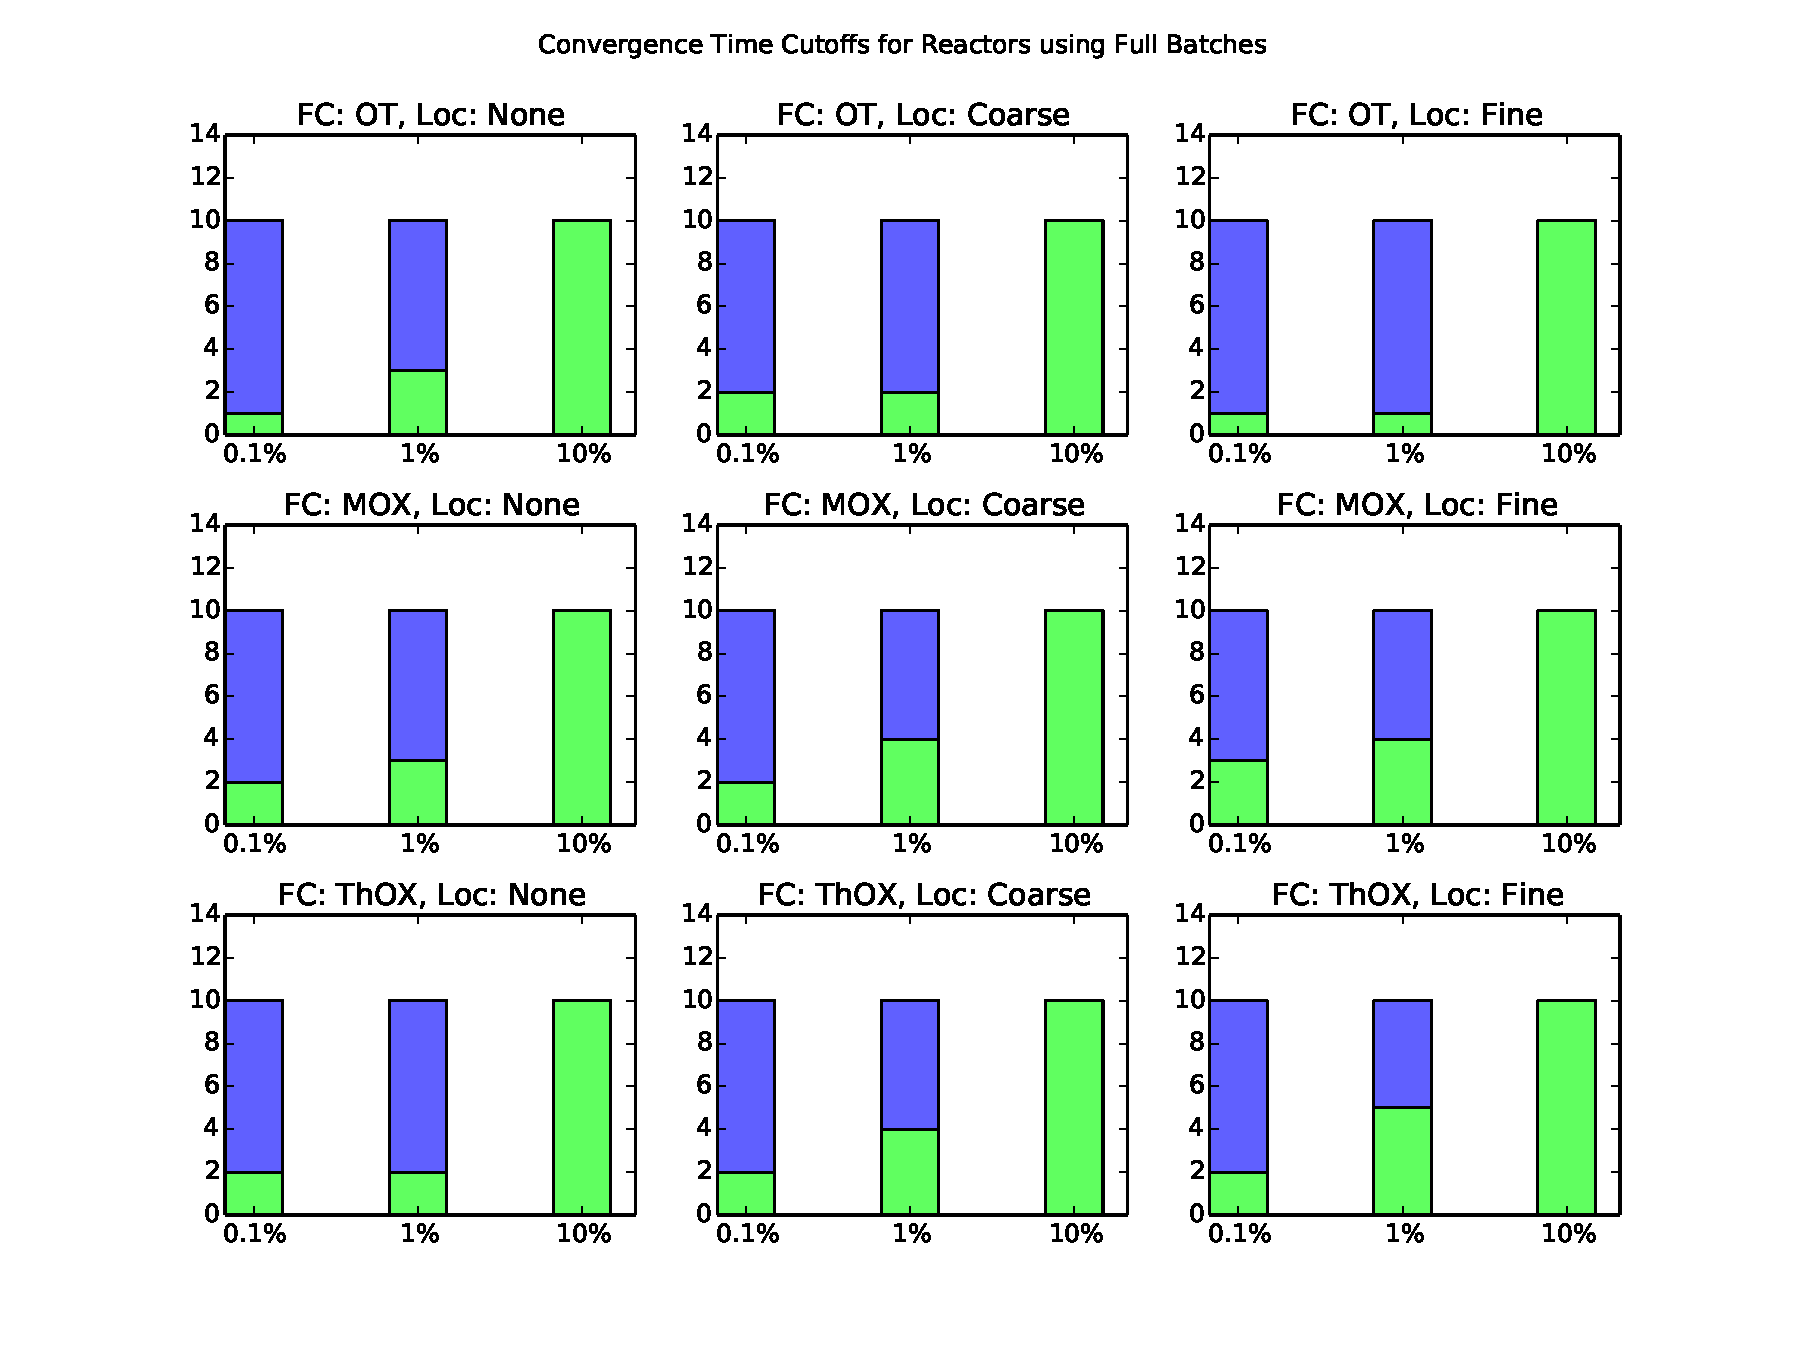
\includegraphics[width=.95\textwidth]{hist_front_rxtr_0.pdf}
    \caption[]{
      \label{fig:hist_front_rxtr_0}
      Effects of increasing convergence criteria on Front-End exchanges with
      reactors exchanging batches. Each bar is divided into how many instances
      converged (green) and did not converge (blue). }
  \end{center}
\end{figure}

\begin{figure}[h!]
  \begin{center}
    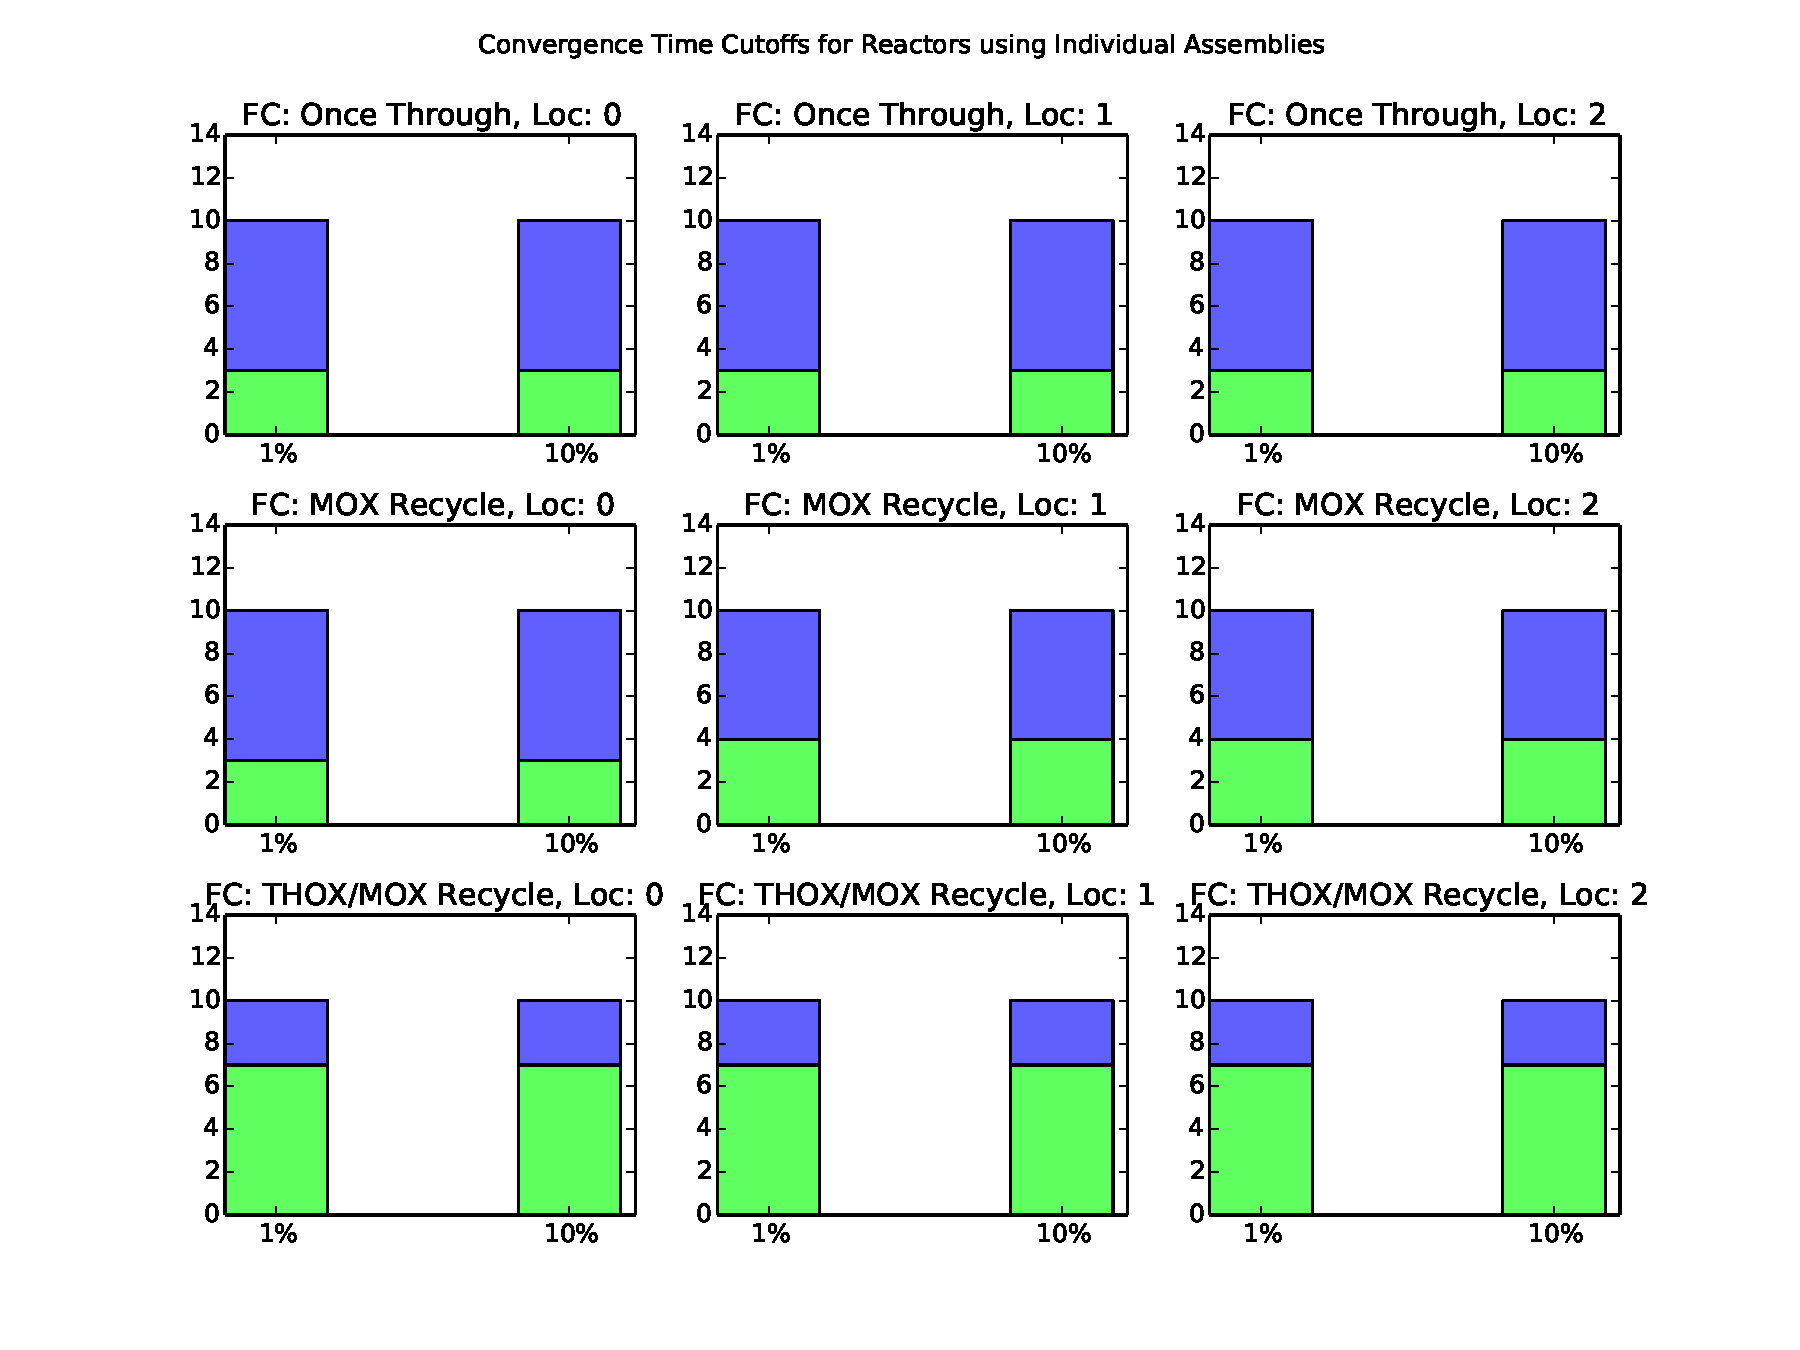
\includegraphics[width=.95\textwidth]{hist_front_rxtr_1.pdf}
    \caption[]{
      \label{fig:hist_front_rxtr_1}
      Effects of increasing convergence criteria on Front-End exchanges with
      reactors exchanging assemblies. Each bar is divided into how many instances
      converged (green) and did not converge (blue).}
  \end{center}
\end{figure}

Unsurprisingly, increasing the convergence criteria for smaller problems has a
greater effect than increasing the convergence criteria for larger probems. It
is somewhat surprising that the increase from a 1\% relative bound gap to a 10\%
gap allows full convergence in the smaller case and has no effect in the larger
case. Users will likely find some relaxation in convergence criteria will
provide speed ups in solution times, as expected. This result seems to indicate
that the relaxed convergence criteria will have a much more profound effect on
smaller problems.

\subsection{Back-End Exchanges}

\subsubsection{Reference Case}



%% \subsubsection{Instance Parameter Variation}
%% % Include large and small r_l_c

%% \paragraph{Location-to-Commodity Importance Ratio}

%% \paragraph{Thermal and Fast-Reactor Populations}

\subsubsection{Convergence Criteria}
